
\begin{landscape}
{\footnotesize
\begin{longtable}{|p{0.13\textwidth}|p{0.11\textwidth}|p{0.09\textwidth}|p{0.09\textwidth}|p{0.11\textwidth}|p{0.13\textwidth}|p{0.13\textwidth}|p{0.09\textwidth}|p{0.09\textwidth}|p{0.04\textwidth}|}
\hline
\textbf{Ratings} & \textbf{Name} & \textbf{Domain} & \textbf{Focus} & \textbf{Keywords} & \textbf{Task Types} & \textbf{AI Capability} & \textbf{Metrics} & \textbf{Models} & \textbf{Citation}  \\ \hline
\endfirsthead
\hline
\textbf{Ratings} & \textbf{Name} & \textbf{Domain} & \textbf{Focus} & \textbf{Keywords} & \textbf{Task Types} & \textbf{AI Capability} & \textbf{Metrics} & \textbf{Models} & \textbf{Citation}  \\ \hline
\endhead
\hline
\multicolumn{10}{r}{Continued on next page} \\
\endfoot
\hline
\endlastfoot
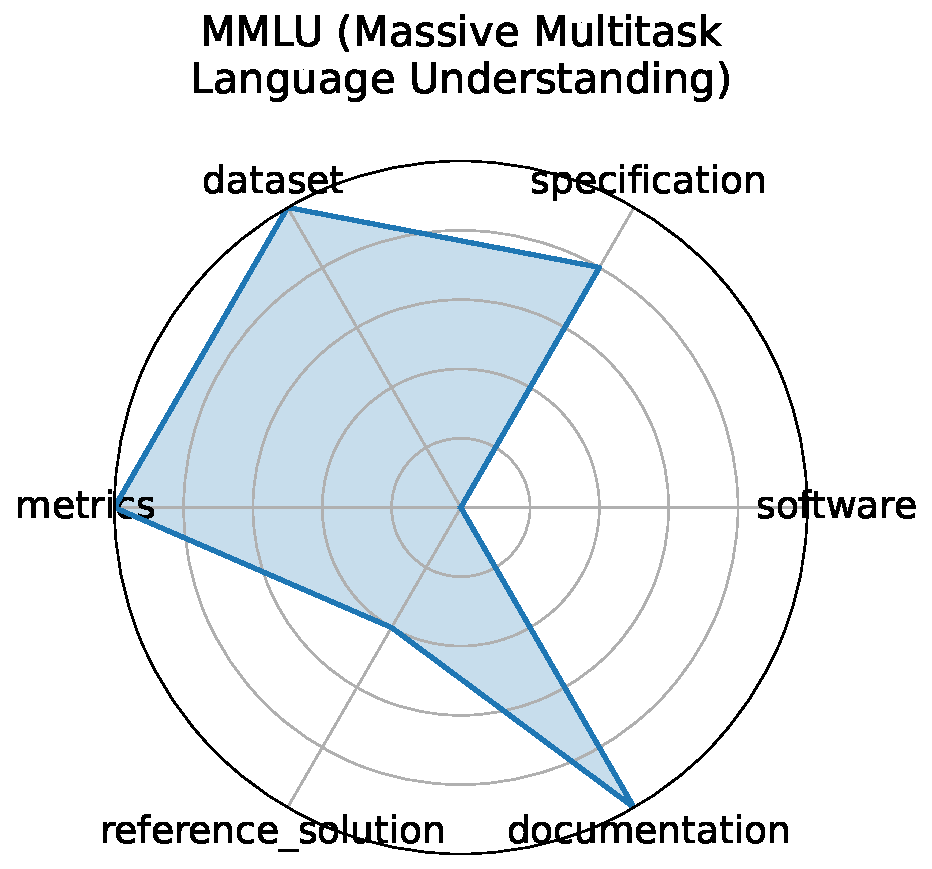
\includegraphics[width=0.15\textwidth]{mmlu_massive_multitask_language_understanding_radar.pdf} & MMLU (Massive Multitask Language Understanding) & Multidomain & Academic knowledge and reasoning across 57 subjects & multitask, multiple-choice, zero-shot, few-shot, knowledge probing & Multiple choice & General reasoning, subject-matter understanding & Accuracy & GPT-4o, Gemini 1.5 Pro, o1, DeepSeek-R1 & \cite{hendrycks2021measuring}\href{https://paperswithcode.com/dataset/mmlu}{$\Rightarrow$} \\ \hline
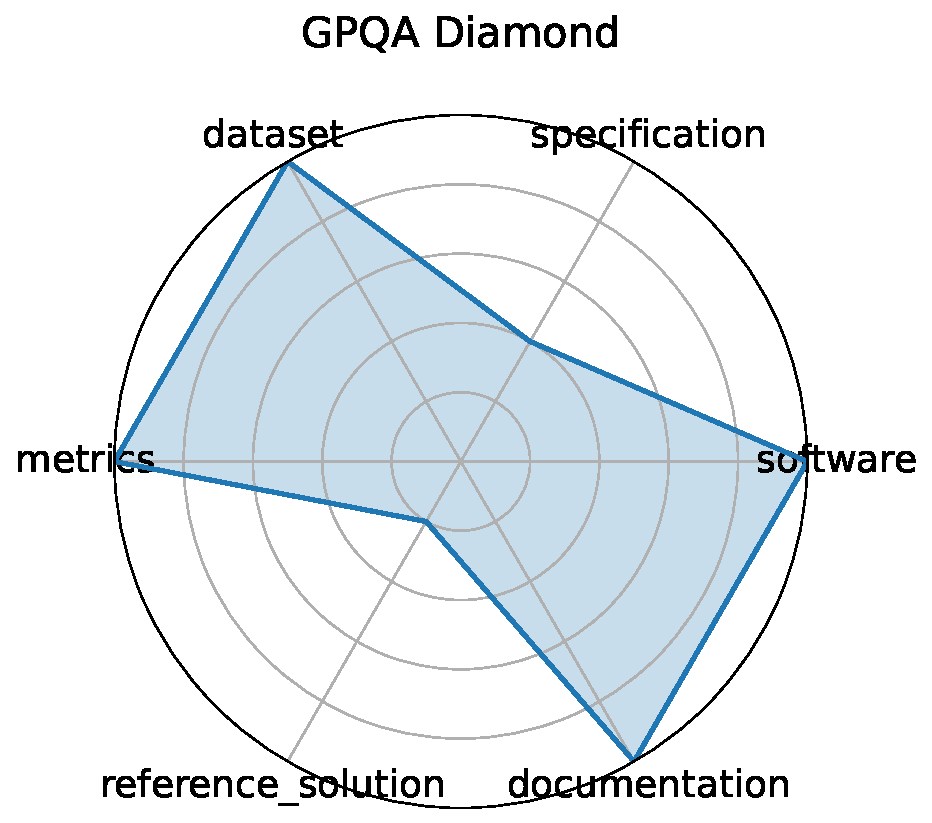
\includegraphics[width=0.15\textwidth]{gpqa_diamond_radar.pdf} & GPQA Diamond & Science & Graduate-level scientific reasoning & Google-proof, graduate-level, science QA, chemistry, physics & Multiple choice, Multi-step QA & Scientific reasoning, deep knowledge & Accuracy & o1, DeepSeek-R1 & \cite{rein2023gpqagraduatelevelgoogleproofqa}\href{https://arxiv.org/abs/2311.12022}{$\Rightarrow$} \\ \hline
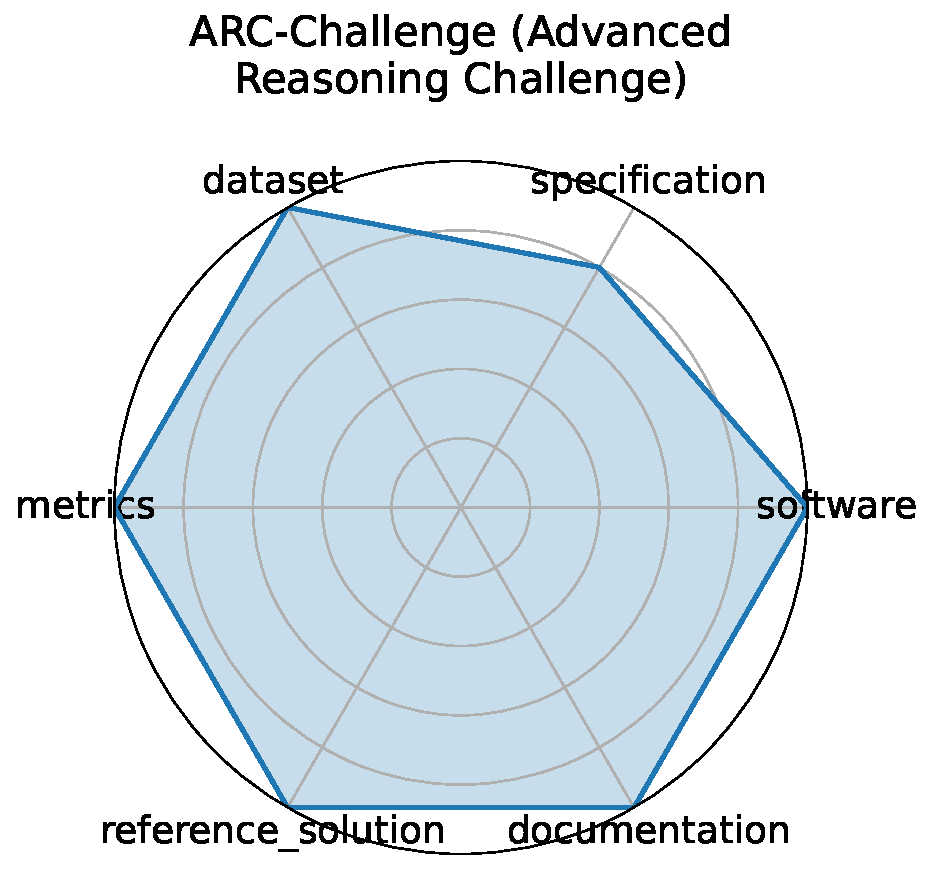
\includegraphics[width=0.15\textwidth]{arc-challenge_advanced_reasoning_challenge_radar.pdf} & ARC-Challenge (Advanced Reasoning Challenge) & Science & Grade-school science with reasoning emphasis & grade-school, science QA, challenge set, reasoning & Multiple choice & Commonsense and scientific reasoning & Accuracy & GPT-4, Claude & \cite{clark2018think}\href{https://allenai.org/data/arc}{$\Rightarrow$} \\ \hline
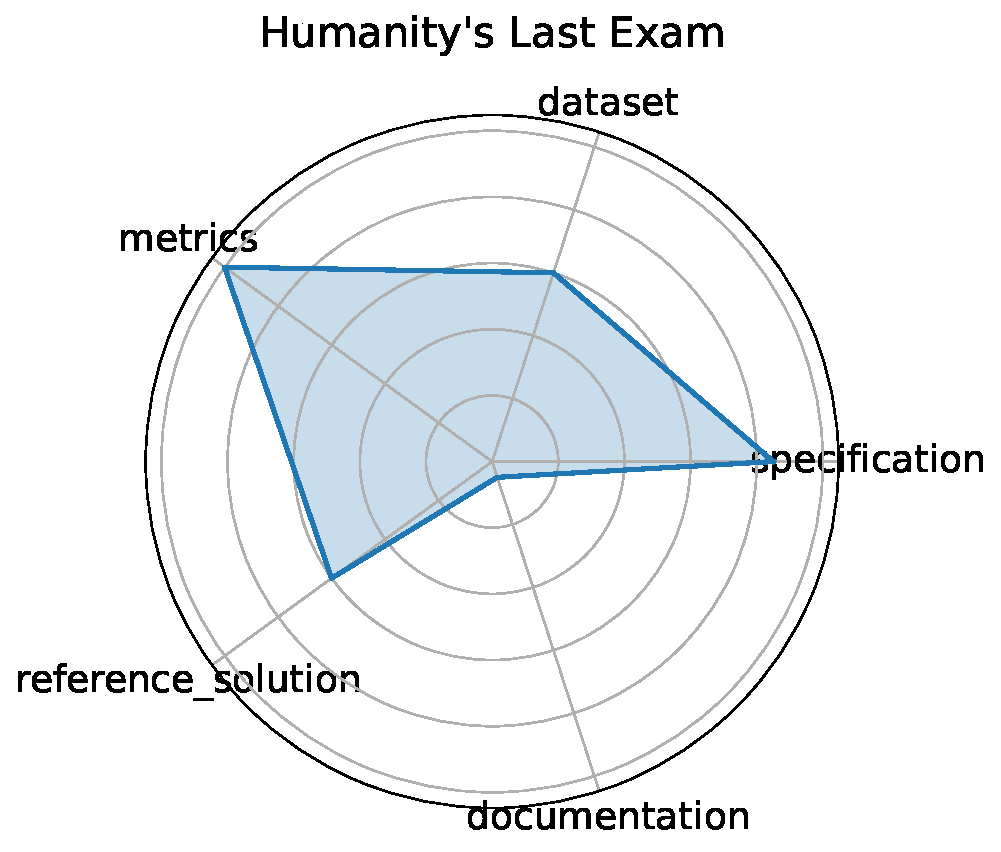
\includegraphics[width=0.15\textwidth]{humanitys_last_exam_radar.pdf} & Humanity's Last Exam & Multidomain & Broad cross-domain academic reasoning & cross-domain, academic exam, multiple-choice, multidisciplinary & Multiple choice & Cross-domain academic reasoning & Accuracy & unkown & \cite{phan2025humanitysexam}\href{https://arxiv.org/abs/2501.14249}{$\Rightarrow$} \\ \hline
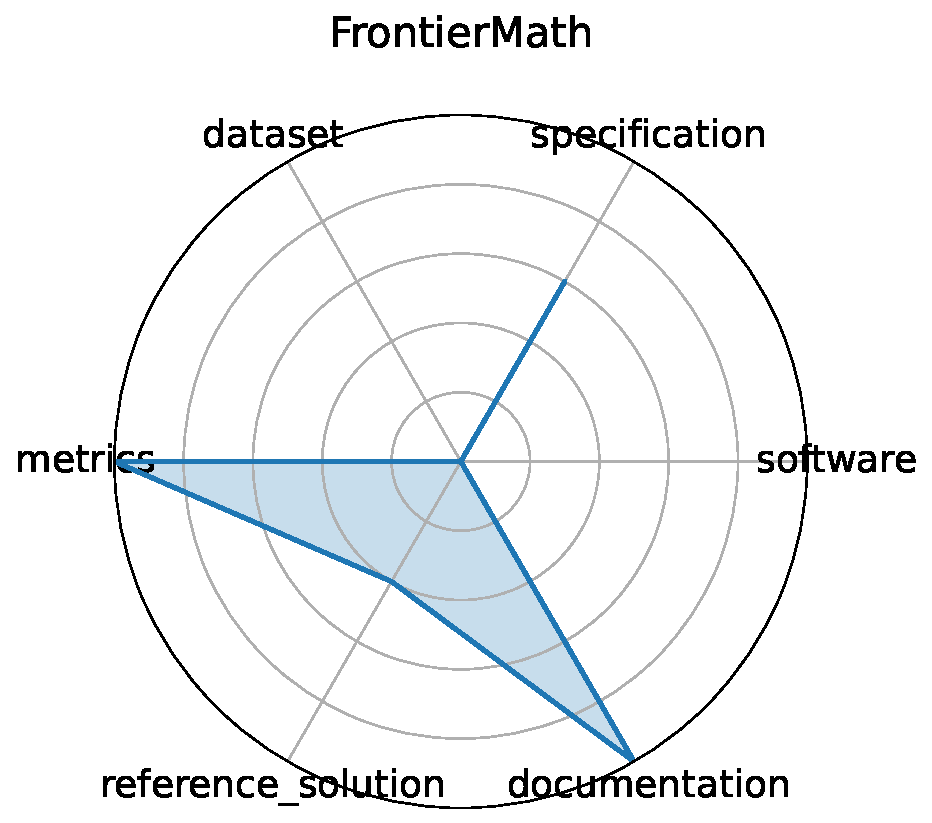
\includegraphics[width=0.15\textwidth]{frontiermath_radar.pdf} & FrontierMath & Mathematics & Challenging advanced mathematical reasoning & symbolic reasoning, number theory, algebraic geometry, category theory & Problem solving & Symbolic and abstract mathematical reasoning & Accuracy & unkown & \cite{glazer2024frontiermathbenchmarkevaluatingadvanced}\href{https://arxiv.org/abs/2411.04872}{$\Rightarrow$} \\ \hline
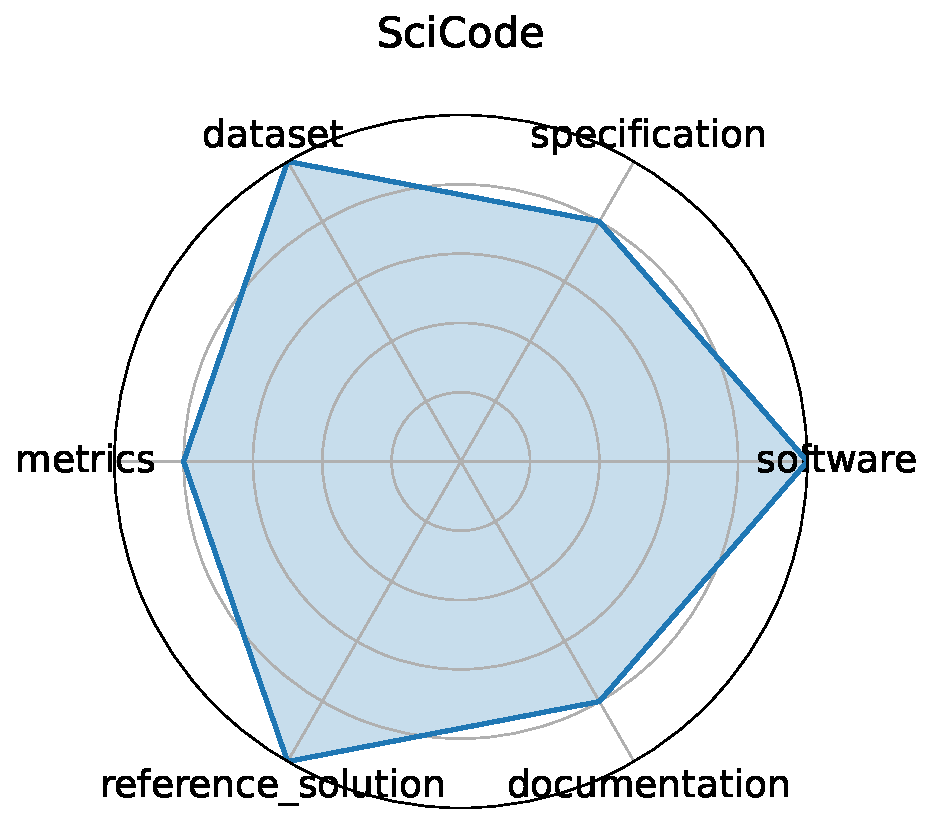
\includegraphics[width=0.15\textwidth]{scicode_radar.pdf} & SciCode & Scientific Programming & Scientific code generation and problem solving & code synthesis, scientific computing, programming benchmark & Coding & Program synthesis, scientific computing & Solve rate (\%) & Claude3.5-Sonnet & \cite{tian2024scicoderesearchcodingbenchmark}\href{https://arxiv.org/abs/2407.13168}{$\Rightarrow$} \\ \hline
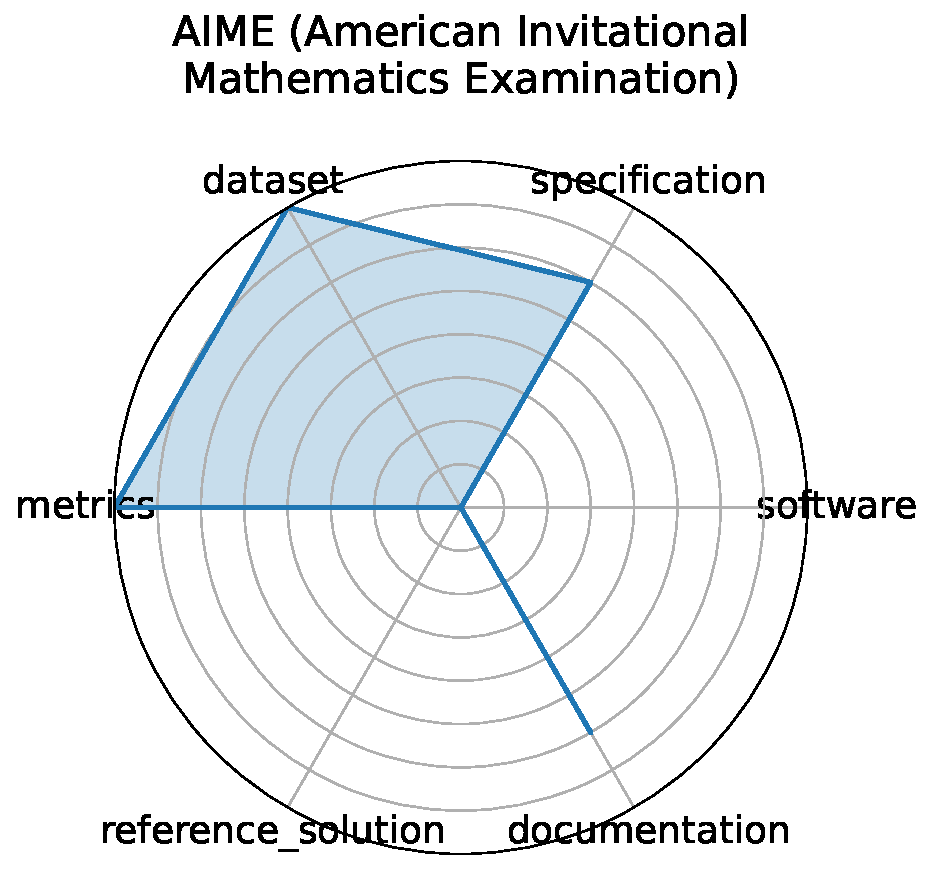
\includegraphics[width=0.15\textwidth]{aime_american_invitational_mathematics_examination_radar.pdf} & AIME (American Invitational Mathematics Examination) & Mathematics & Pre-college advanced problem solving & algebra, combinatorics, number theory, geometry & Problem solving & Mathematical problem-solving and reasoning & Accuracy & unkown & \cite{www-aime}\href{https://artofproblemsolving.com/wiki/index.php/AIME\_Problems\_and\_Solutions}{$\Rightarrow$} \\ \hline
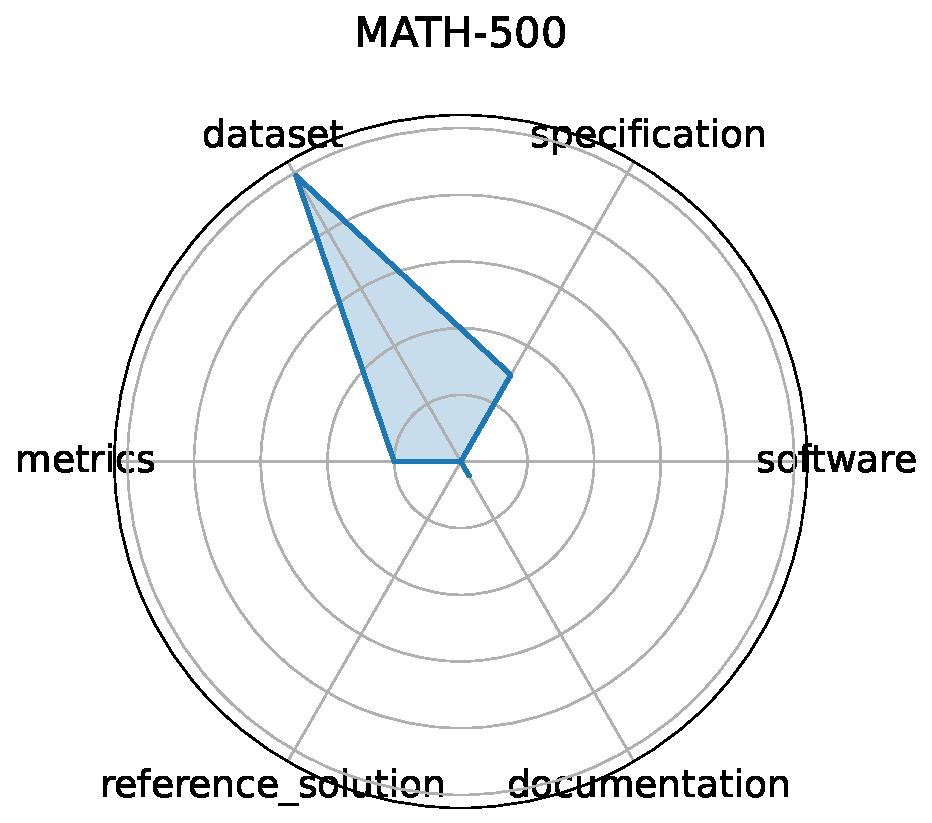
\includegraphics[width=0.15\textwidth]{math-_radar.pdf} & MATH-500 & Mathematics & Math reasoning generalization & calculus, algebra, number theory, geometry & Problem solving & Math reasoning and generalization & Accuracy & unkown & \cite{huggingface2025math500}\href{https://huggingface.co/datasets/HuggingFaceH4/MATH-500}{$\Rightarrow$} \\ \hline
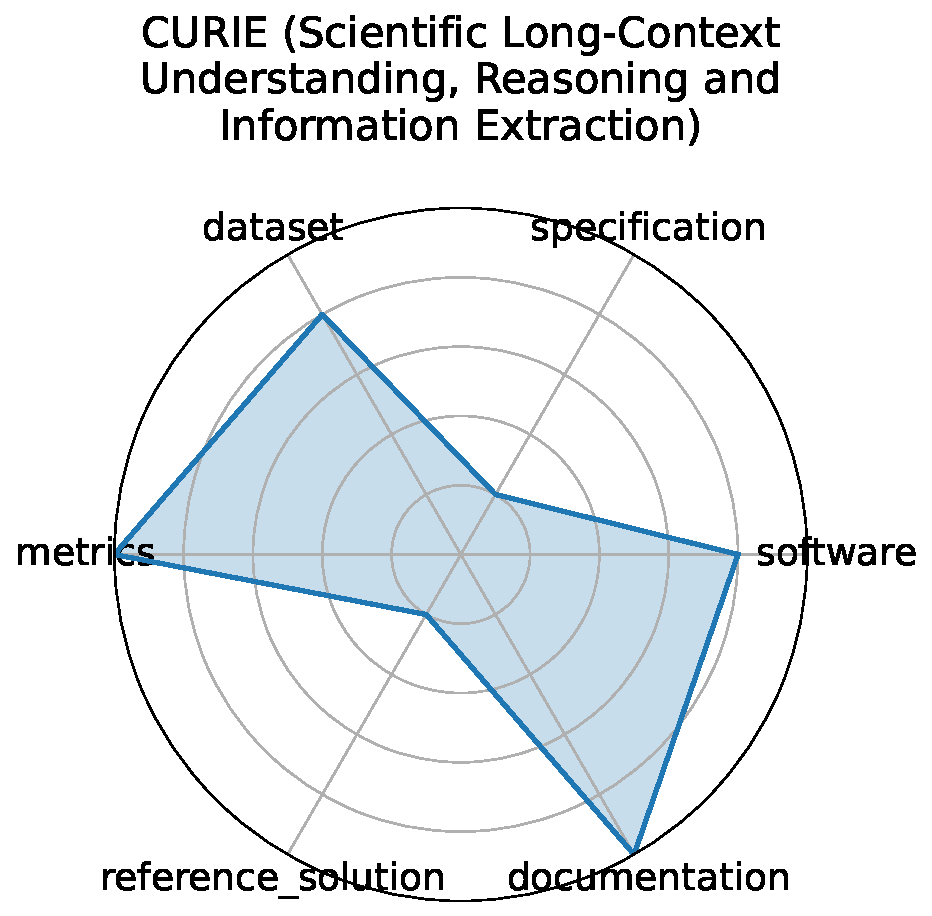
\includegraphics[width=0.15\textwidth]{curie_scientific_long-context_understanding_reasoning_and_information_extraction_radar.pdf} & CURIE (Scientific Long-Context Understanding, Reasoning and Information Extraction) & Multidomain Science & Long-context scientific reasoning & long-context, information extraction, multimodal & Information extraction, Reasoning, Concept tracking, Aggregation, Algebraic manipulation, Multimodal comprehension & Long-context understanding and scientific reasoning & Accuracy & unkown & \cite{cui2025curieevaluatingllmsmultitask}\href{https://arxiv.org/abs/2503.13517}{$\Rightarrow$} \\ \hline
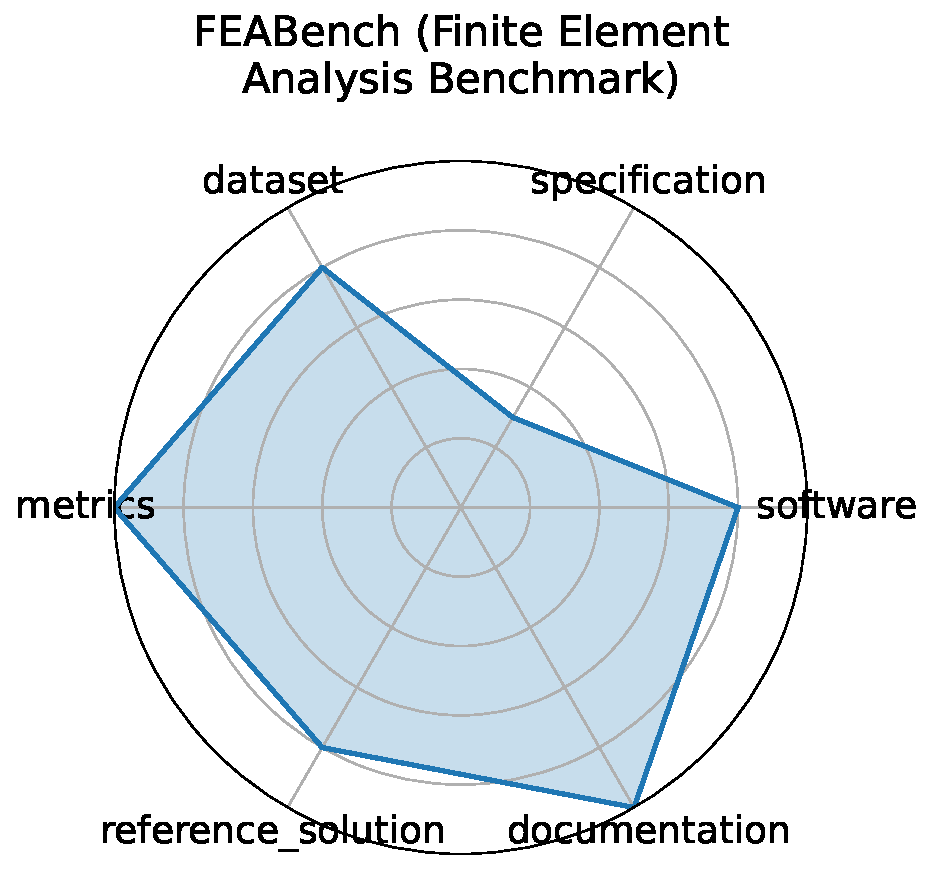
\includegraphics[width=0.15\textwidth]{feabench_finite_element_analysis_benchmark_radar.pdf} & FEABench (Finite Element Analysis Benchmark) & Computational Engineering & FEA simulation accuracy and performance & finite element, simulation, PDE & Simulation, Performance evaluation & Numerical simulation accuracy and efficiency & Solve time, Error norm & FEniCS, deal.II & \cite{mudur2025feabenchevaluatinglanguagemodels}\href{https://github.com/google/feabench}{$\Rightarrow$} \\ \hline
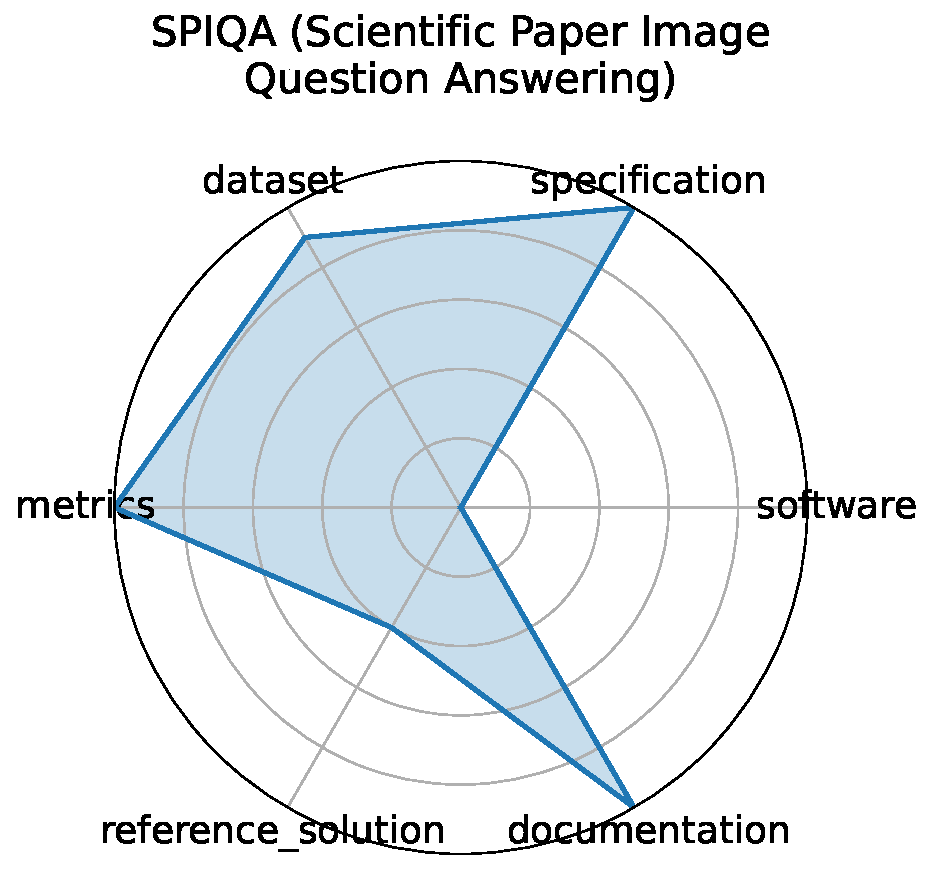
\includegraphics[width=0.15\textwidth]{spiqa_scientific_paper_image_question_answering_radar.pdf} & SPIQA (Scientific Paper Image Question Answering) & Computer Science & Multimodal QA on scientific figures & multimodal QA, figure understanding, table comprehension, chain-of-thought & Question answering, Multimodal QA, Chain-of-Thought evaluation & Visual-textual reasoning in scientific contexts & Accuracy, F1 score & Chain-of-Thought models, Multimodal QA systems & \cite{zhong2024spiqa}\href{https://arxiv.org/abs/2407.09413}{$\Rightarrow$} \\ \hline
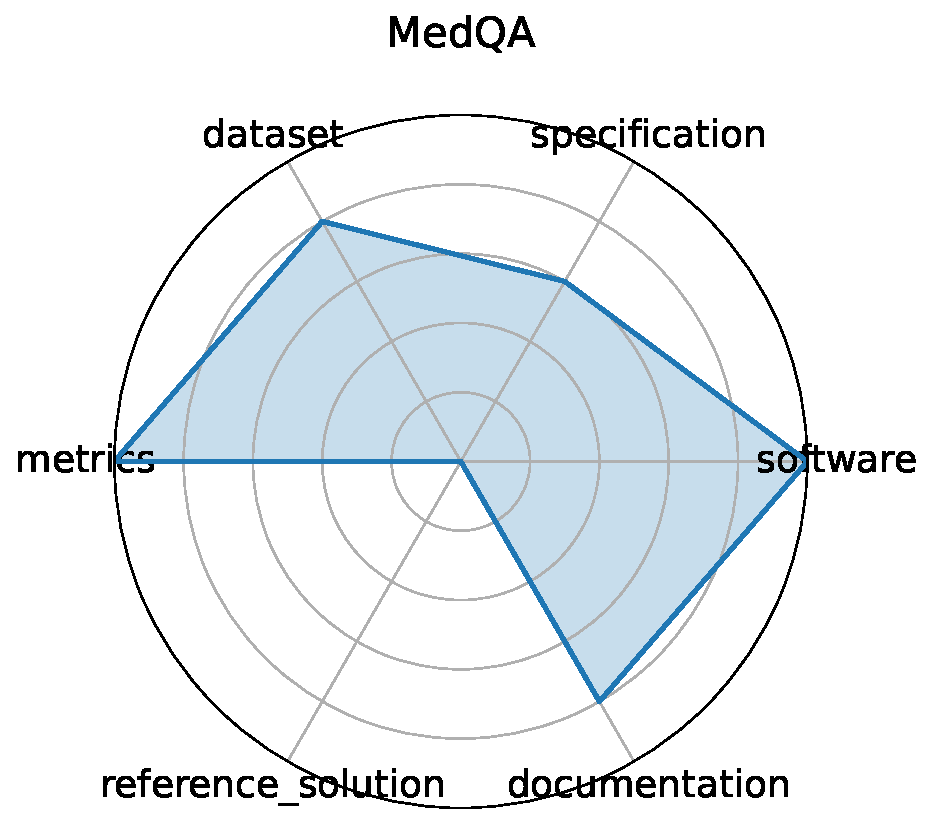
\includegraphics[width=0.15\textwidth]{medqa_radar.pdf} & MedQA & Medical Question Answering & Medical board exam QA & USMLE, diagnostic QA, medical knowledge, multilingual & Multiple choice & Medical diagnosis and knowledge retrieval & Accuracy & Neural reader, Retrieval-based QA systems & \cite{jin2020diseasedoespatienthave}\href{https://arxiv.org/abs/2009.13081}{$\Rightarrow$} \\ \hline
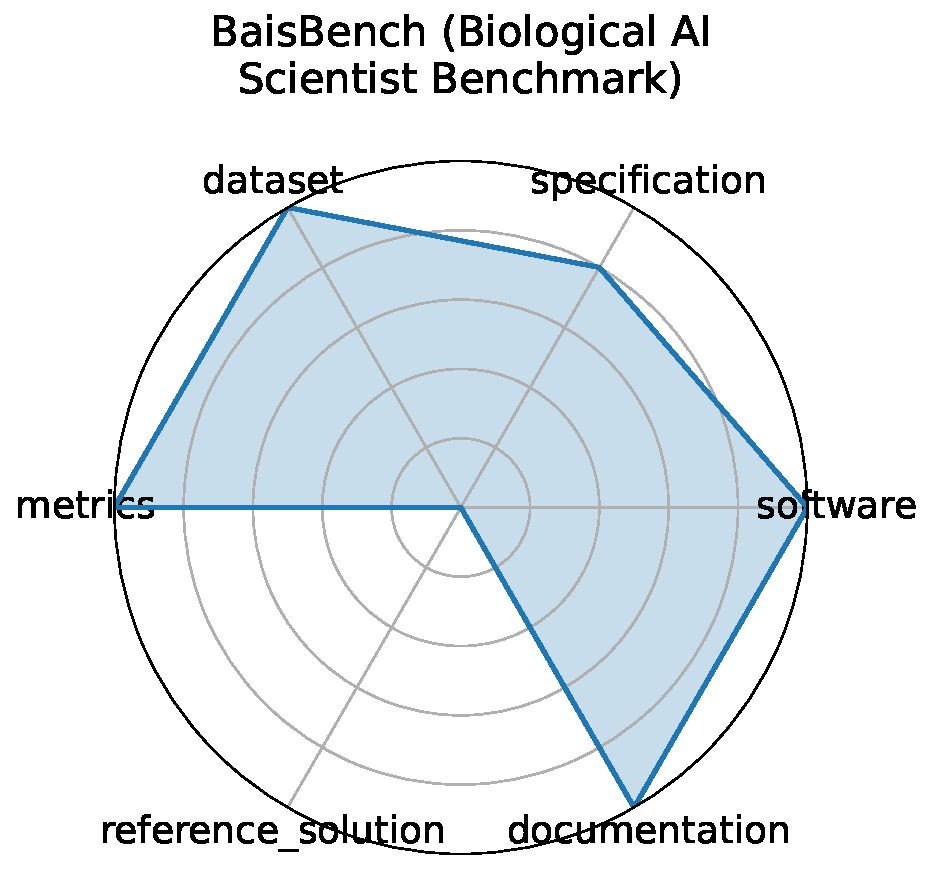
\includegraphics[width=0.15\textwidth]{baisbench_biological_ai_scientist_benchmark_radar.pdf} & BaisBench (Biological AI Scientist Benchmark) & Computational Biology & Omics-driven AI research tasks & single-cell annotation, biological QA, autonomous discovery & Cell type annotation, Multiple choice & Autonomous biological research capabilities & Annotation accuracy, QA accuracy & LLM-based AI scientist agents & \cite{luo2025benchmarkingaiscientistsomics}\href{https://arxiv.org/abs/2505.08341}{$\Rightarrow$} \\ \hline
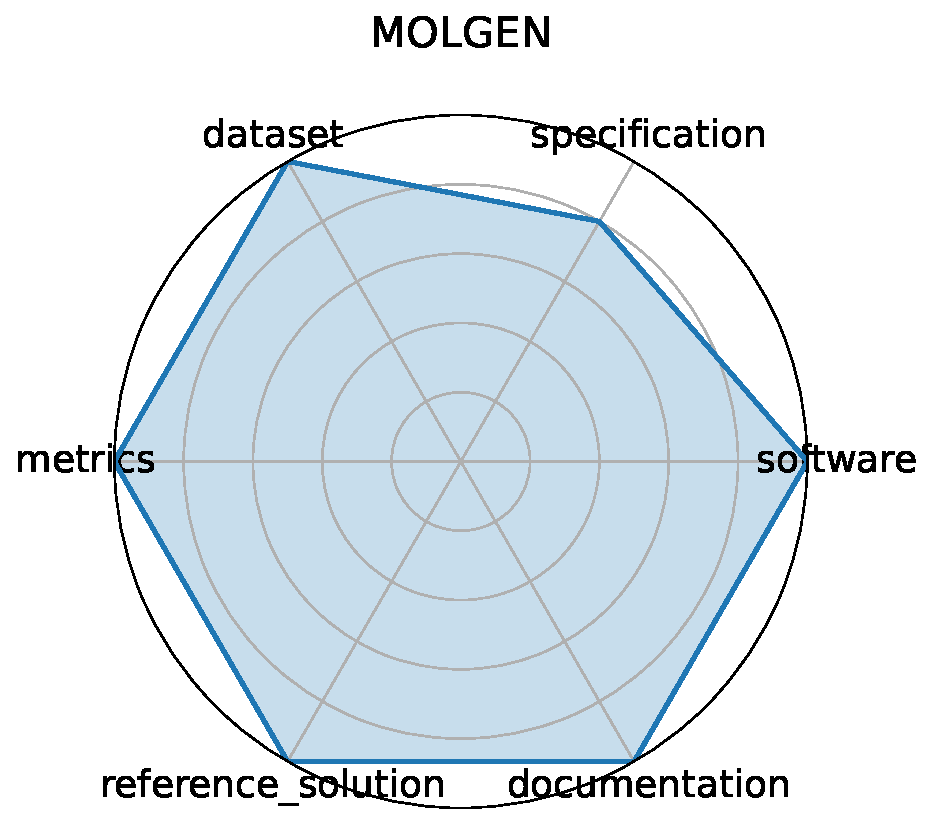
\includegraphics[width=0.15\textwidth]{molgen_radar.pdf} & MOLGEN & Computational Chemistry & Molecular generation and optimization & SELFIES, GAN, property optimization & Distribution learning, Goal-oriented generation & Generation of valid and optimized molecular structures & Validity\%, Novelty\%, QED, Docking score & MolGen & \cite{fang2024domainagnosticmoleculargenerationchemical}\href{https://github.com/zjunlp/MolGen}{$\Rightarrow$} \\ \hline
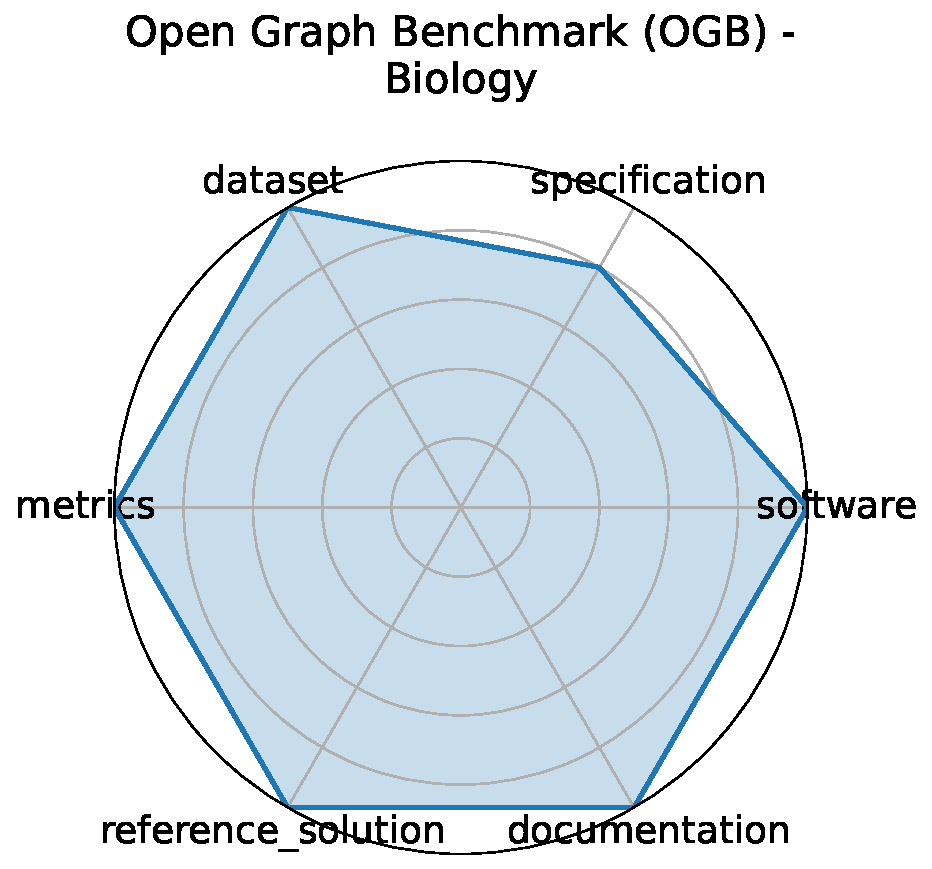
\includegraphics[width=0.15\textwidth]{open_graph_benchmark_ogb_-_biology_radar.pdf} & Open Graph Benchmark (OGB) - Biology & Graph ML & Biological graph property prediction & node prediction, link prediction, graph classification & Node property prediction, Link property prediction, Graph property prediction & Scalability and generalization in graph ML for biology & Accuracy, ROC-AUC & GCN, GraphSAGE, GAT & \cite{hu2021opengraphbenchmarkdatasets}\href{https://ogb.stanford.edu/docs/home/}{$\Rightarrow$} \\ \hline
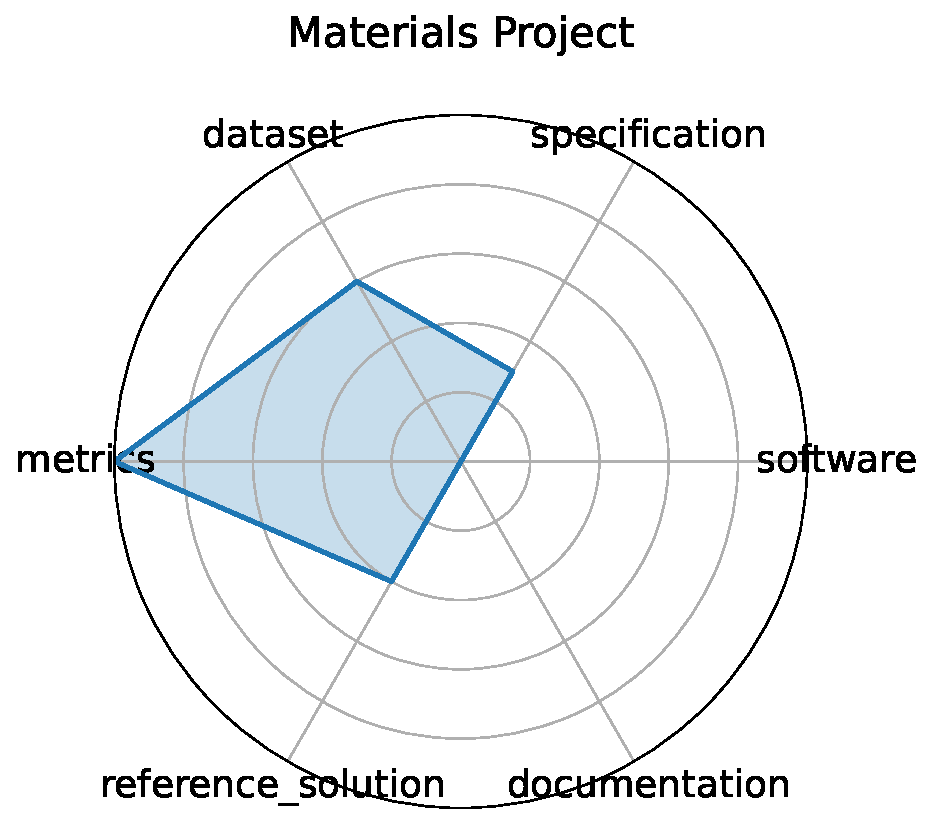
\includegraphics[width=0.15\textwidth]{materials_project_radar.pdf} & Materials Project & Materials Science & DFT-based property prediction & DFT, materials genome, high-throughput & Property prediction & Prediction of inorganic material properties & MAE, R{\textasciicircum}2 & Automatminer, Crystal Graph Neural Networks & \cite{jain2013materials}\href{https://materialsproject.org/}{$\Rightarrow$} \\ \hline
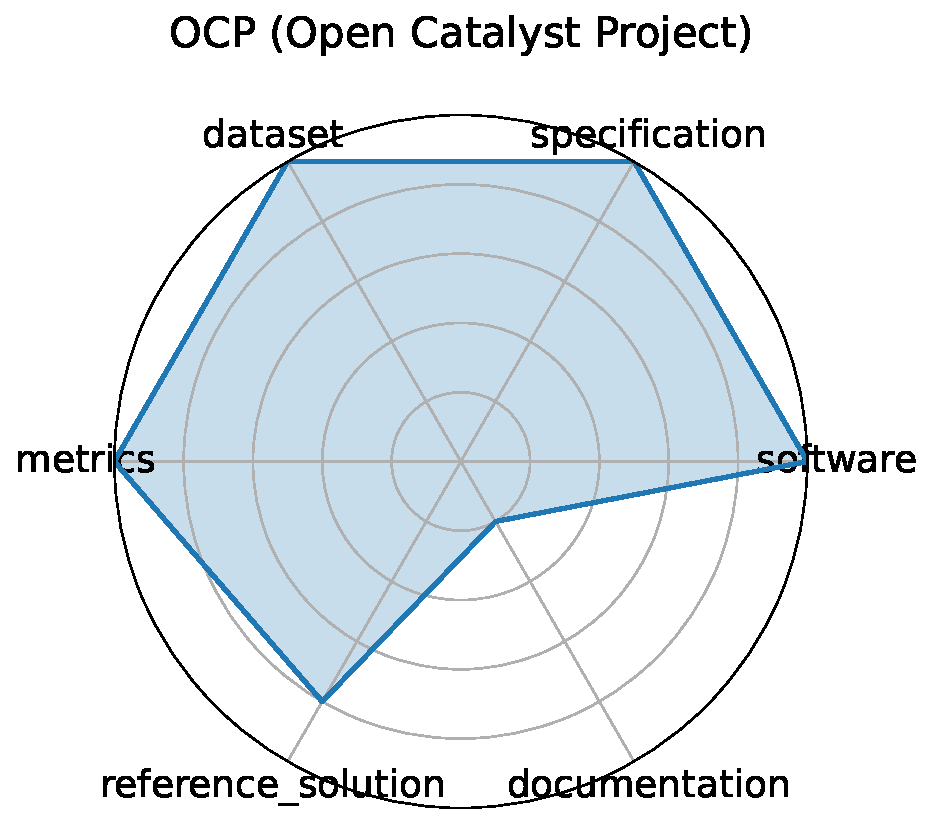
\includegraphics[width=0.15\textwidth]{ocp_open_catalyst_project_radar.pdf} & OCP (Open Catalyst Project) & Chemistry; Materials Science & Catalyst adsorption energy prediction & DFT relaxations, adsorption energy, graph neural networks & Energy prediction, Force prediction & Prediction of adsorption energies and forces & MAE (energy), MAE (force) & CGCNN, SchNet, DimeNet++, GemNet-OC & \cite{chanussot2021oc20,tran2023oc22,doi:10.1021/acscatal.0c04525,tran2023b}\href{https://opencatalystproject.org/}{$\Rightarrow$} \\ \hline
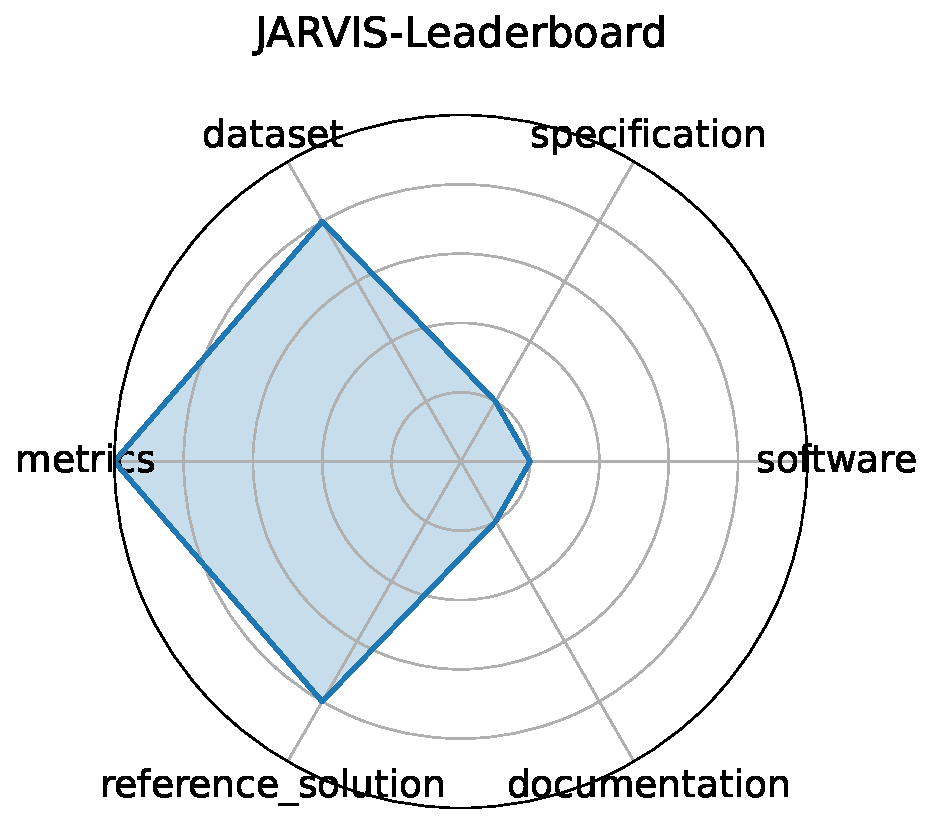
\includegraphics[width=0.15\textwidth]{jarvis-leaderboard_radar.pdf} & JARVIS-Leaderboard & Materials Science; Benchmarking & Comparative evaluation of materials design methods & leaderboards, materials methods, simulation & Method benchmarking, Leaderboard ranking & Performance comparison across diverse materials design methods & MAE, RMSE, Accuracy & unkown & \cite{choudhary2024jarvis}\href{https://arxiv.org/abs/2306.11688}{$\Rightarrow$} \\ \hline
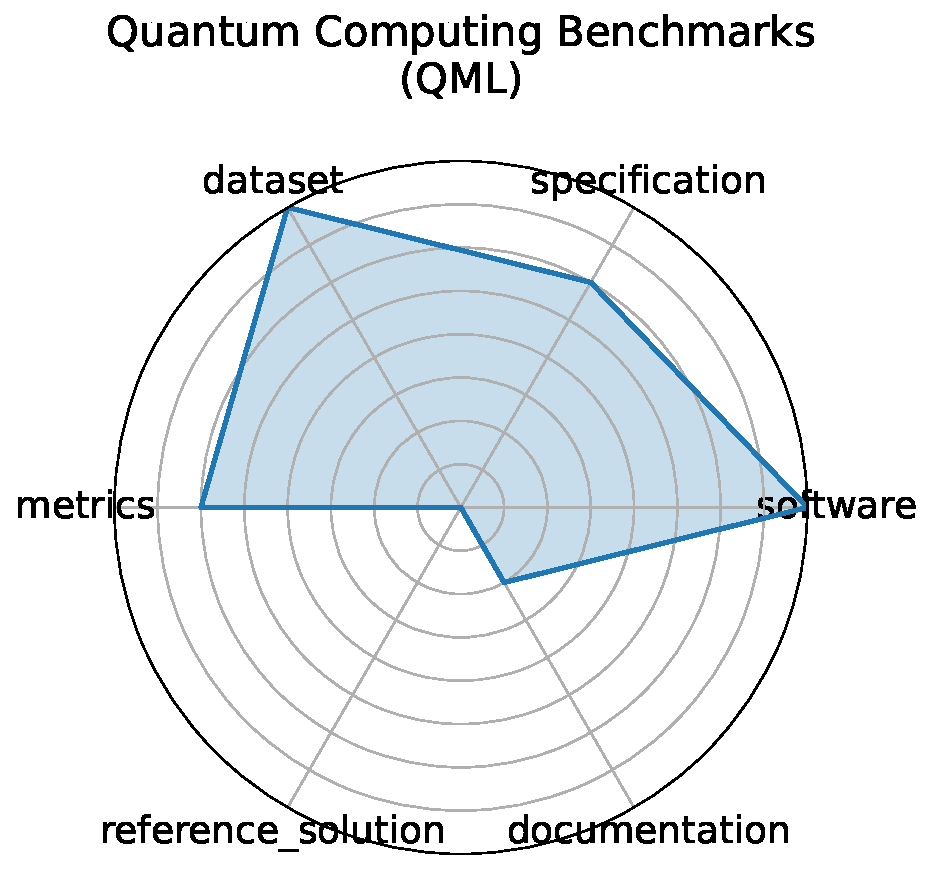
\includegraphics[width=0.15\textwidth]{quantum_computing_benchmarks_qml_radar.pdf} & Quantum Computing Benchmarks (QML) & Quantum Computing & Quantum algorithm performance evaluation & quantum circuits, state preparation, error correction & Circuit benchmarking, State classification & Quantum algorithm performance and fidelity & Fidelity, Success probability & IBM Q, IonQ, AQT@LBNL & \cite{kiwit2023}\href{https://github.com/XanaduAI/qml-benchmarks}{$\Rightarrow$} \\ \hline
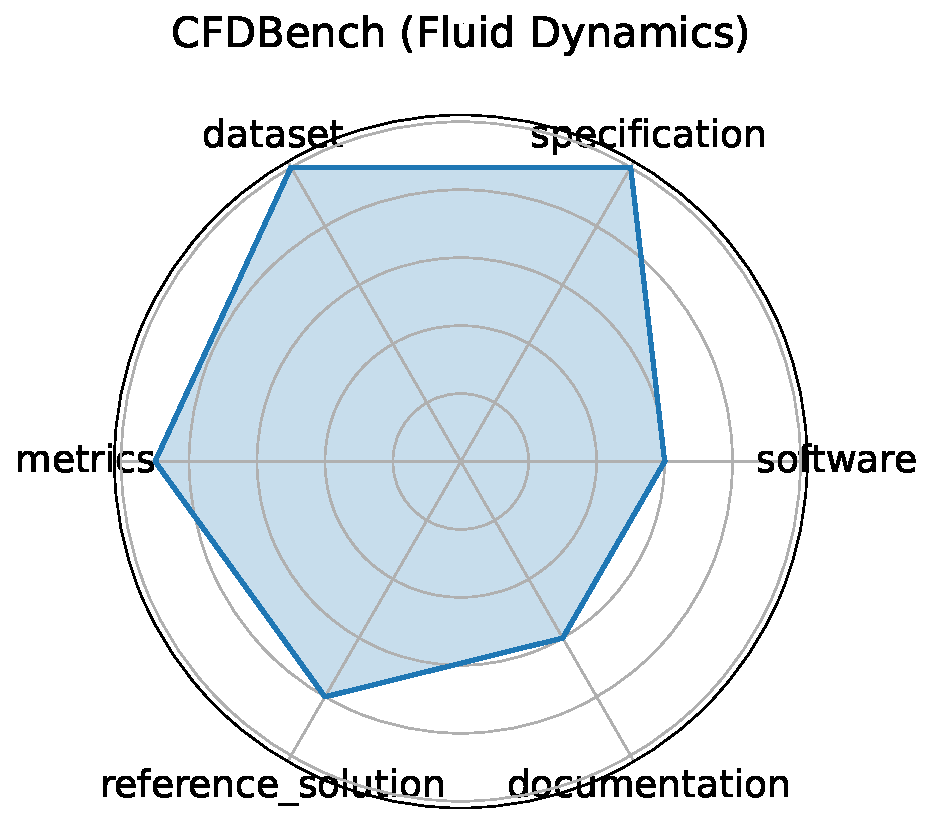
\includegraphics[width=0.15\textwidth]{cfdbench_fluid_dynamics_radar.pdf} & CFDBench (Fluid Dynamics) & Fluid Dynamics; Scientific ML & Neural operator surrogate modeling & neural operators, CFD, FNO, DeepONet & Surrogate modeling & Generalization of neural operators for PDEs & L2 error, MAE & FNO, DeepONet, U-Net & \cite{luo2024cfdbenchlargescalebenchmarkmachine}\href{https://arxiv.org/abs/2310.05963}{$\Rightarrow$} \\ \hline
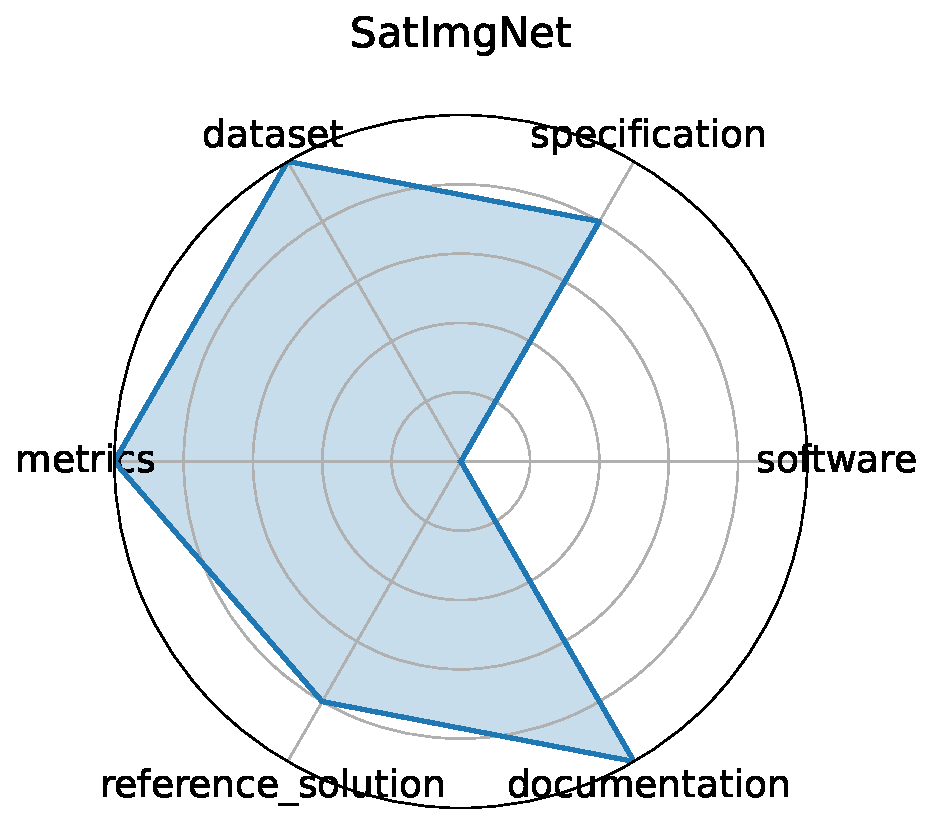
\includegraphics[width=0.15\textwidth]{satimgnet_radar.pdf} & SatImgNet & Remote Sensing & Satellite imagery classification & land-use, zero-shot, multi-task & Image classification & Zero-shot land-use classification & Accuracy & CLIP, BLIP, ALBEF & \cite{roberts2023satin}\href{https://huggingface.co/datasets/saral-ai/satimagnet}{$\Rightarrow$} \\ \hline
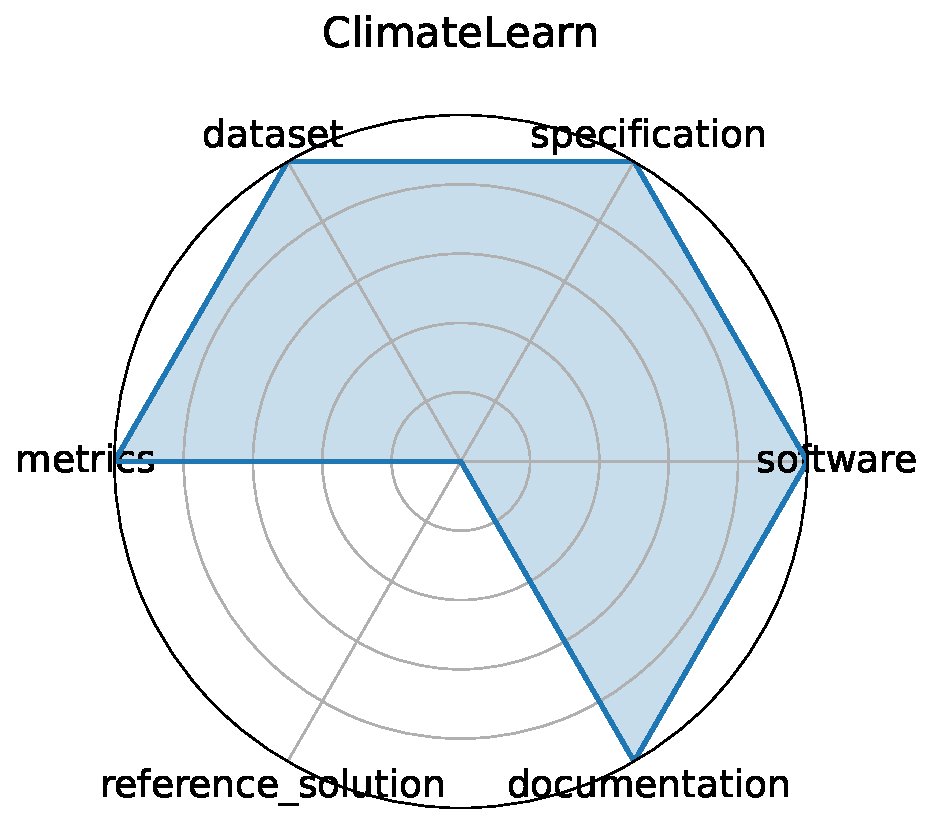
\includegraphics[width=0.15\textwidth]{climatelearn_radar.pdf} & ClimateLearn & Climate Science; Forecasting & ML for weather and climate modeling & medium-range forecasting, ERA5, data-driven & Forecasting & Global weather prediction (3-5 days) & RMSE, Anomaly correlation & CNN baselines, ResNet variants & \cite{nguyen2023climatelearnbenchmarkingmachinelearning}\href{https://arxiv.org/abs/2307.01909}{$\Rightarrow$} \\ \hline
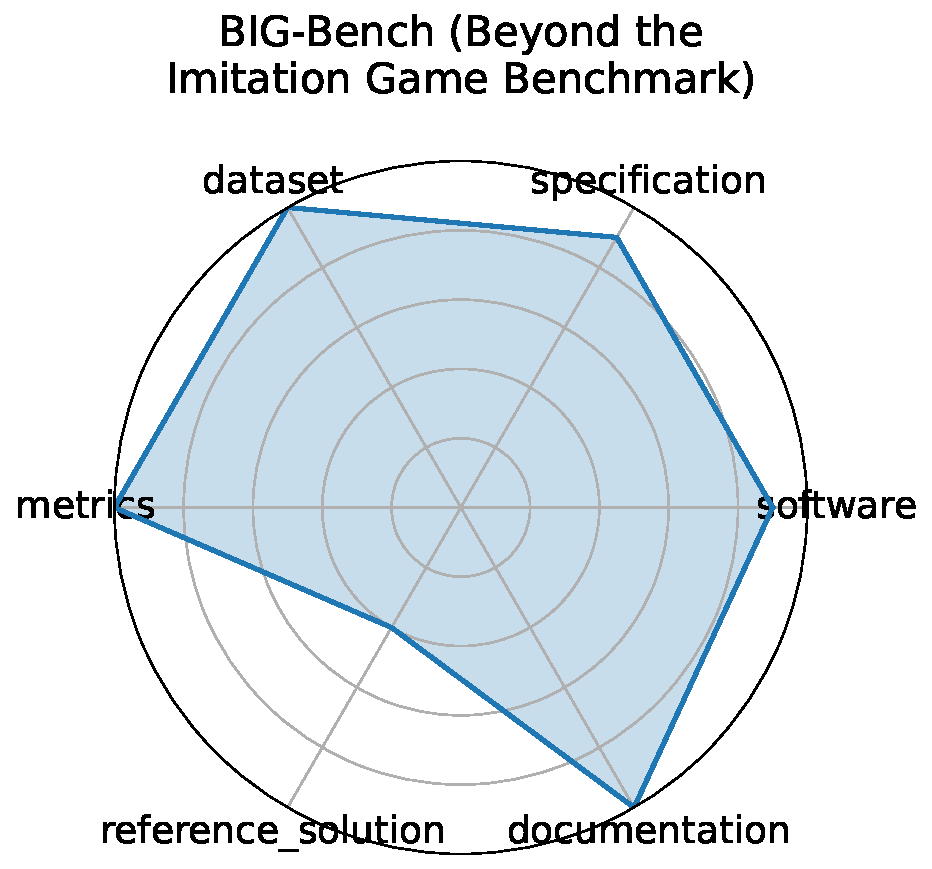
\includegraphics[width=0.15\textwidth]{big-bench_beyond_the_imitation_game_benchmark_radar.pdf} & BIG-Bench (Beyond the Imitation Game Benchmark) & NLP; AI Evaluation & Diverse reasoning and generalization tasks & few-shot, multi-task, bias analysis & Few-shot evaluation, Multi-task evaluation & Reasoning and generalization across diverse tasks & Accuracy, Task-specific metrics & GPT-3, Dense Transformers, Sparse Transformers & \cite{srivastava2023imitationgamequantifyingextrapolating}\href{https://github.com/google/BIG-bench}{$\Rightarrow$} \\ \hline
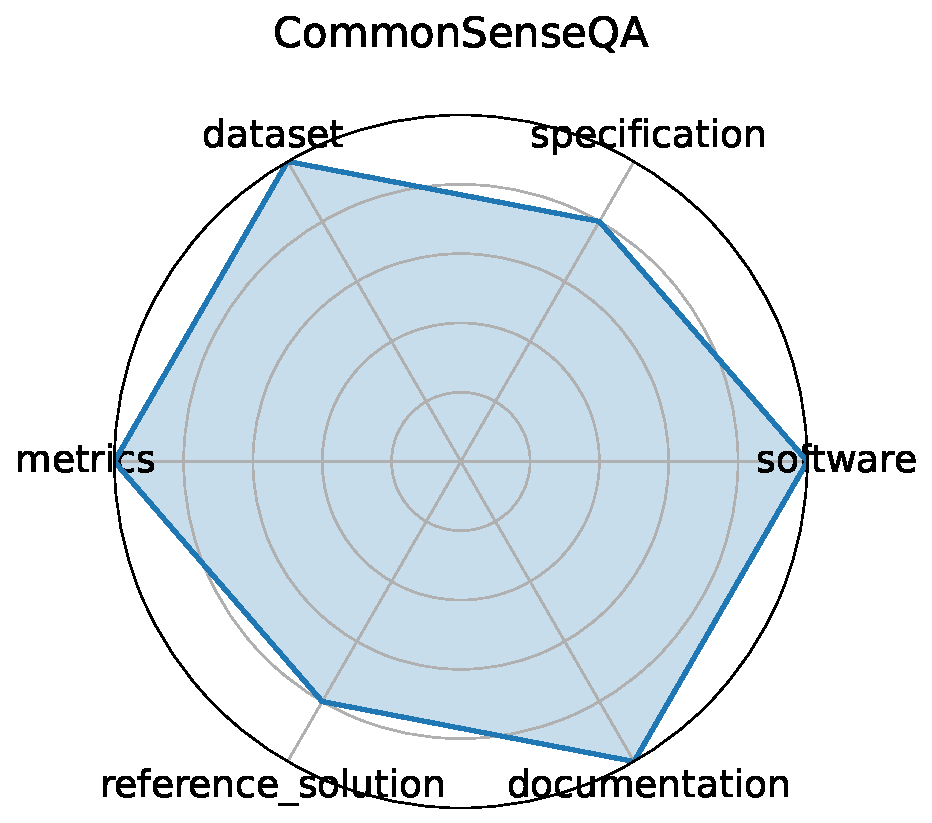
\includegraphics[width=0.15\textwidth]{commonsenseqa_radar.pdf} & CommonSenseQA & NLP; Commonsense & Commonsense question answering & ConceptNet, multiple-choice, adversarial & Multiple choice & Commonsense reasoning and knowledge integration & Accuracy & BERT-large, RoBERTa, GPT-3 & \cite{talmor2019commonsenseqaquestionansweringchallenge}\href{https://paperswithcode.com/paper/commonsenseqa-a-question-answering-challenge}{$\Rightarrow$} \\ \hline
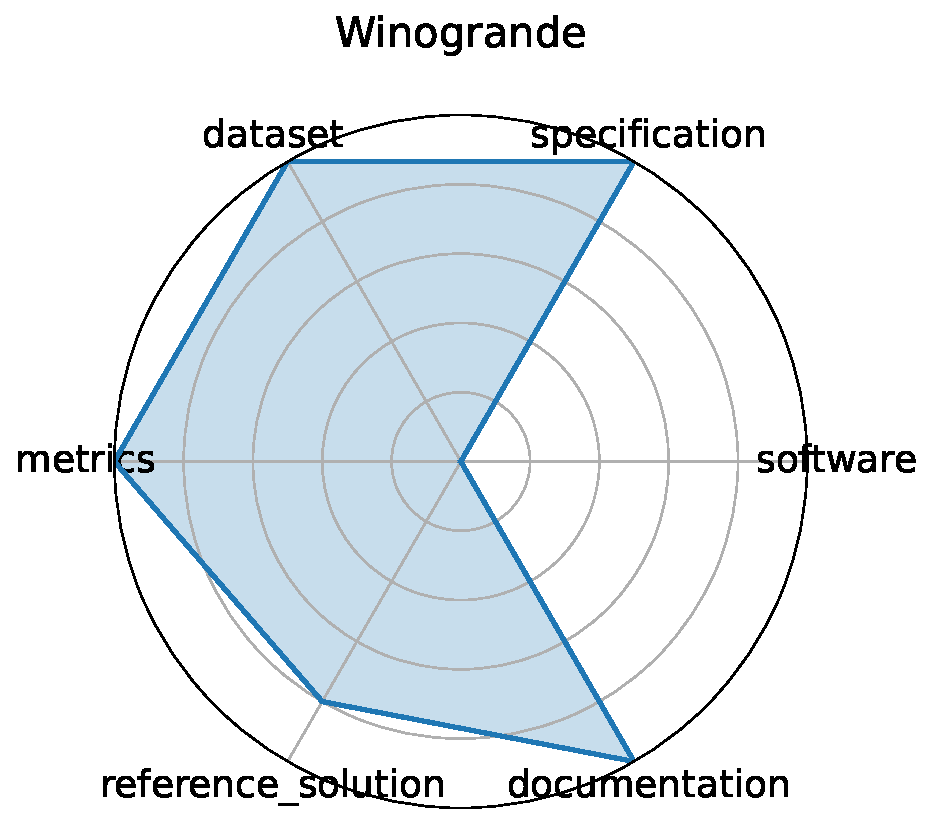
\includegraphics[width=0.15\textwidth]{winogrande_radar.pdf} & Winogrande & NLP; Commonsense & Winograd Schema-style pronoun resolution & adversarial, pronoun resolution & Pronoun resolution & Robust commonsense reasoning & Accuracy, AUC & RoBERTa, BERT, GPT-2 & \cite{sakaguchi2019winograndeadversarialwinogradschema}\href{https://leaderboard.allenai.org/winogrande/submissions/public}{$\Rightarrow$} \\ \hline
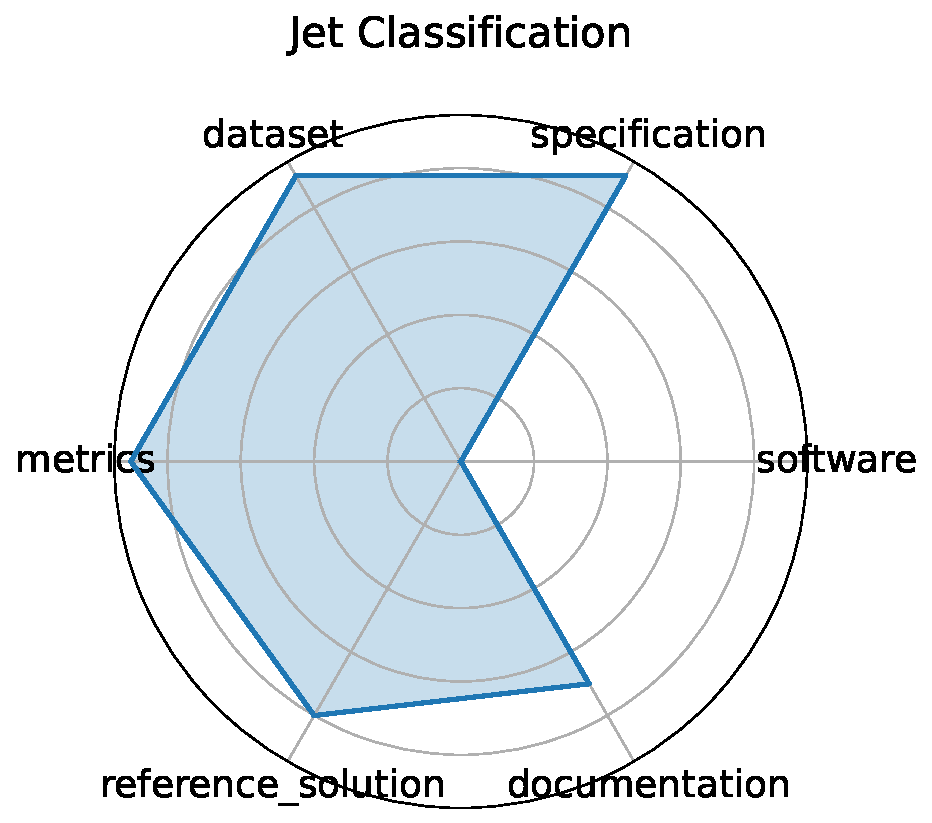
\includegraphics[width=0.15\textwidth]{jet_classification_radar.pdf} & Jet Classification & Particle Physics & Real-time classification of particle jets using HL-LHC simulation features & classification, real-time ML, jet tagging, QKeras & Classification & Real-time inference, model compression performance & Accuracy, AUC & Keras DNN, QKeras quantized DNN & \cite{duarte2022fastml}\href{https://github.com/fastmachinelearning/fastml-science/tree/main/jet-classify}{$\Rightarrow$} \\ \hline
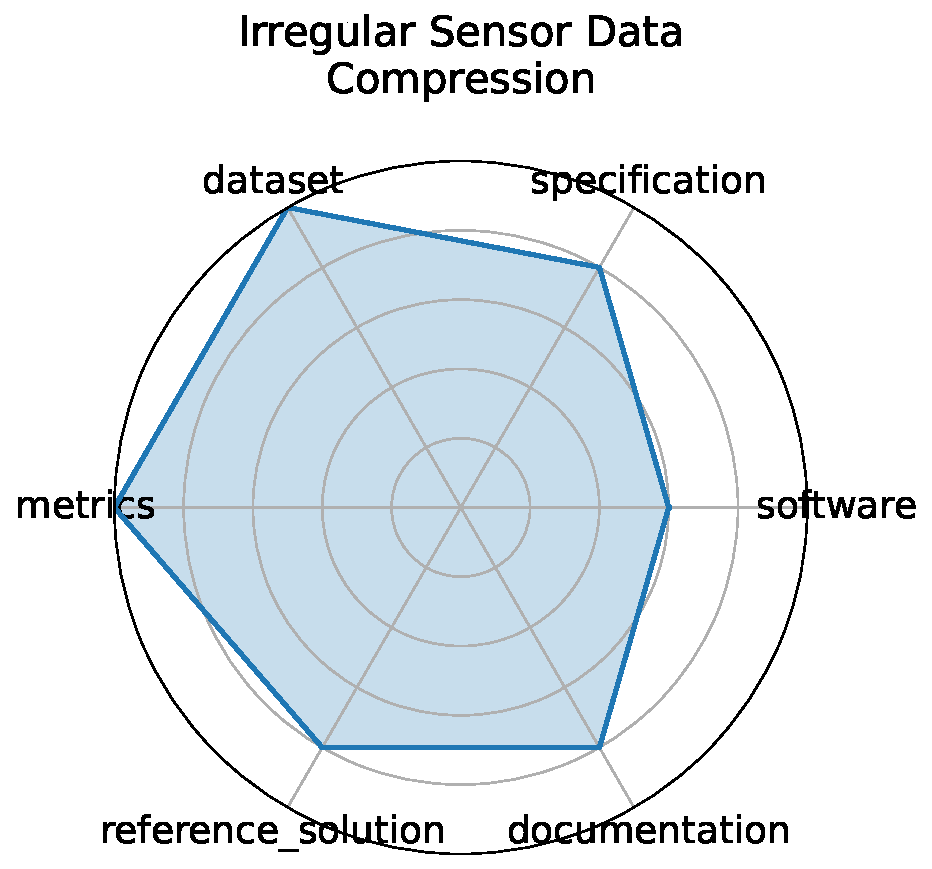
\includegraphics[width=0.15\textwidth]{irregular_sensor_data_compression_radar.pdf} & Irregular Sensor Data Compression & Particle Physics & Real-time compression of sparse sensor data with autoencoders & compression, autoencoder, sparse data, irregular sampling & Compression & Reconstruction quality, compression efficiency & MSE, Compression ratio & Autoencoder, Quantized autoencoder & \cite{duarte2022fastmlsciencebenchmarksaccelerating2}\href{https://github.com/fastmachinelearning/fastml-science/tree/main/sensor-data-compression}{$\Rightarrow$} \\ \hline
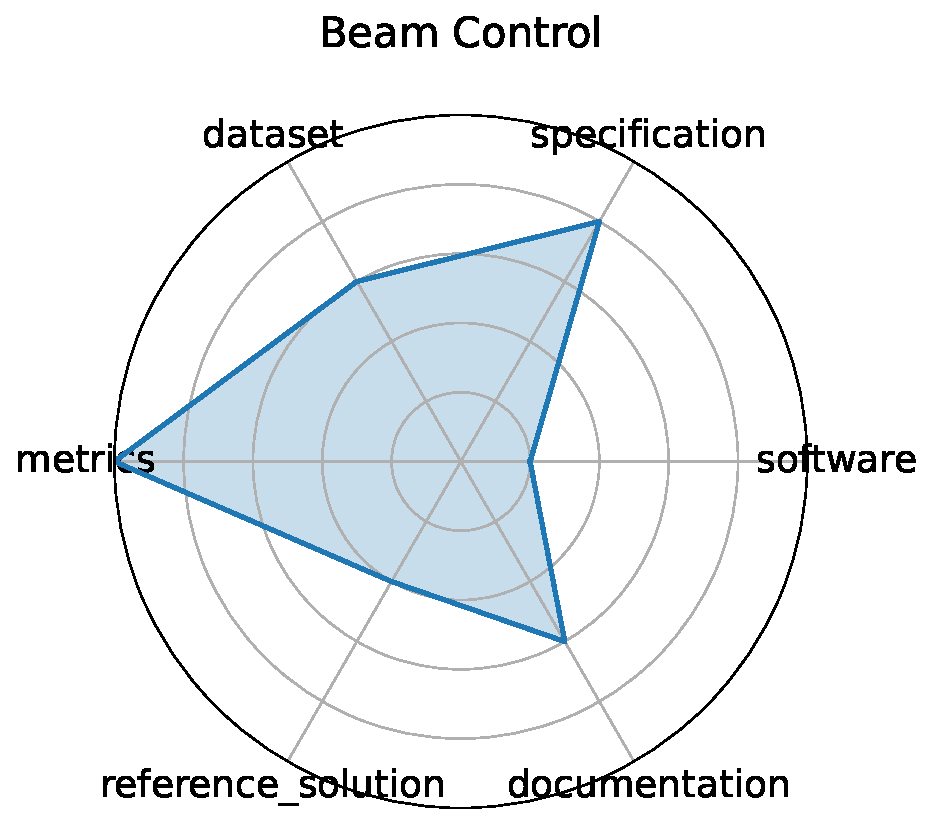
\includegraphics[width=0.15\textwidth]{beam_control_radar.pdf} & Beam Control & Accelerators and Magnets & Reinforcement learning control of accelerator beam position & RL, beam stabilization, control systems, simulation & Control & Policy performance in simulated accelerator control & Stability, Control loss & DDPG, PPO (planned) & \cite{duarte2022fastmlsciencebenchmarksaccelerating3,kafkes2021boostrdatasetacceleratorcontrol}\href{https://github.com/fastmachinelearning/fastml-science/tree/main/beam-control}{$\Rightarrow$} \\ \hline
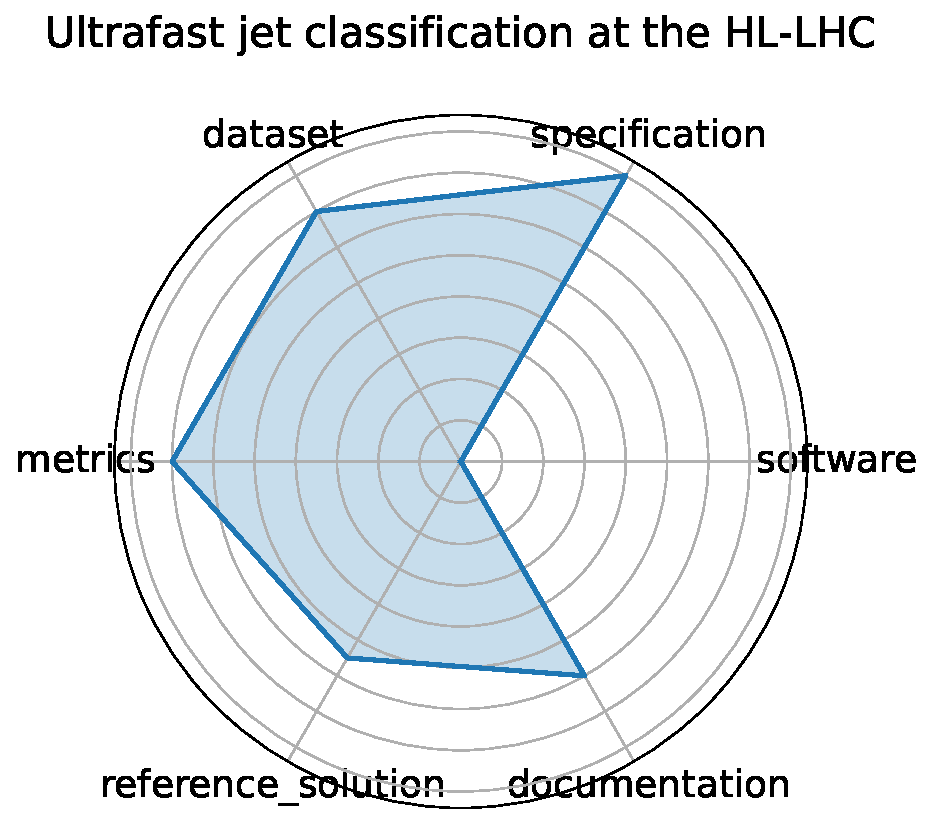
\includegraphics[width=0.15\textwidth]{ultrafast_jet_classification_at_the_hl-lhc_radar.pdf} & Ultrafast jet classification at the HL-LHC & Particle Physics & FPGA-optimized real-time jet origin classification at the HL-LHC & jet classification, FPGA, quantization-aware training, Deep Sets, Interaction Networks & Classification & Real-time inference under FPGA constraints & Accuracy, Latency, Resource utilization & MLP, Deep Sets, Interaction Network & \cite{odagiu2024ultrafastjetclassificationfpgas}\href{https://arxiv.org/pdf/2402.01876}{$\Rightarrow$} \\ \hline
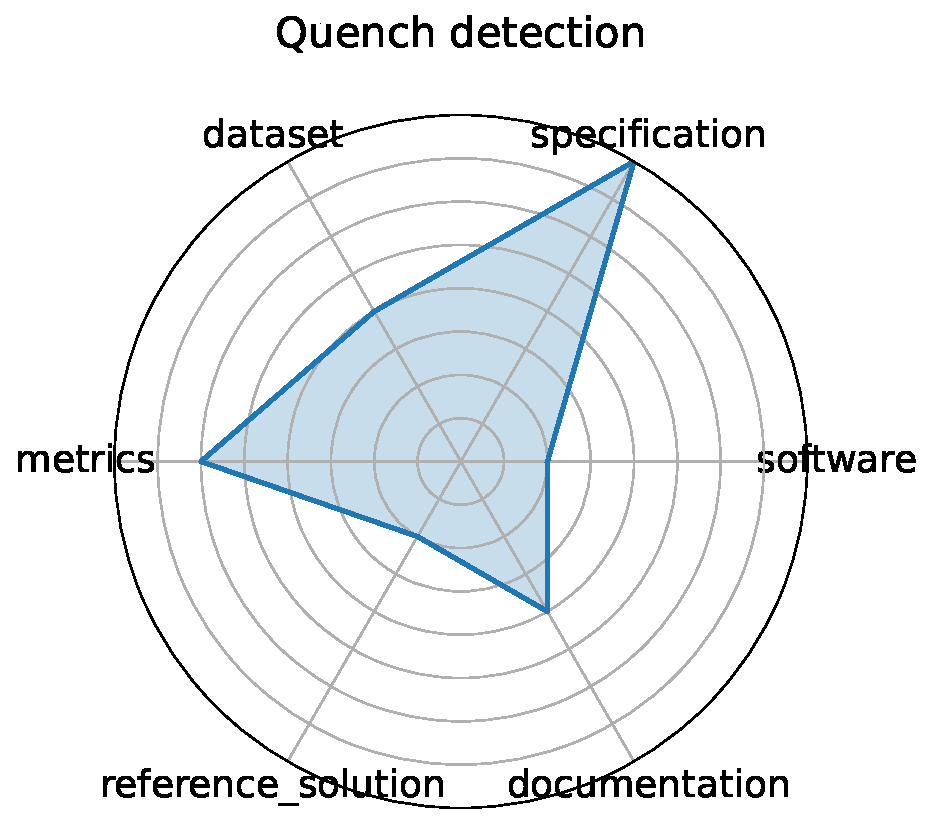
\includegraphics[width=0.15\textwidth]{quench_detection_radar.pdf} & Quench detection & Accelerators and Magnets & Real-time detection of superconducting magnet quenches using ML & quench detection, autoencoder, anomaly detection, real-time & Anomaly detection, Quench localization & Real-time anomaly detection with multi-modal sensors & ROC-AUC, Detection latency & Autoencoder, RL agents (in development) & \cite{quench2024}\href{https://indico.cern.ch/event/1387540/contributions/6153618/attachments/2948441/5182077/fast\_ml\_magnets\_2024\_final.pdf}{$\Rightarrow$} \\ \hline
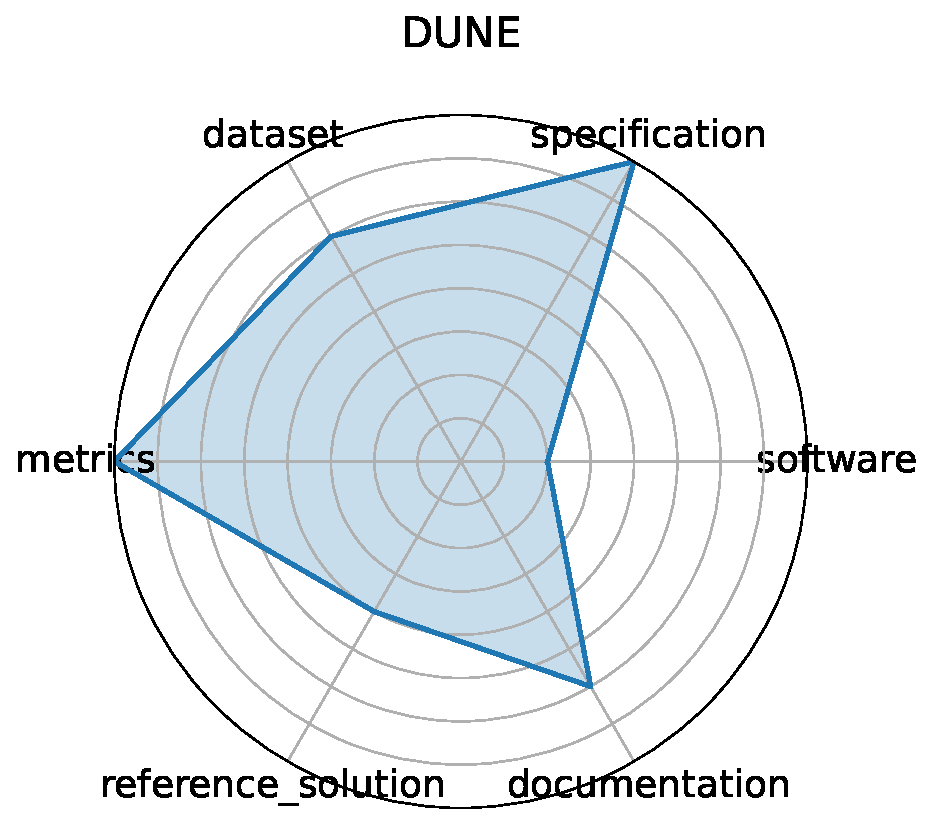
\includegraphics[width=0.15\textwidth]{dune_radar.pdf} & DUNE & Particle Physics & Real-time ML for DUNE DAQ time-series data & DUNE, time-series, real-time, trigger & Trigger selection, Time-series anomaly detection & Low-latency event detection & Detection efficiency, Latency & CNN, LSTM (planned) & \cite{abud2021deep}\href{https://indico.fnal.gov/event/66520/contributions/301423/attachments/182439/250508/fast\_ml\_dunedaq\_sonic\_10\_15\_24.pdf}{$\Rightarrow$} \\ \hline
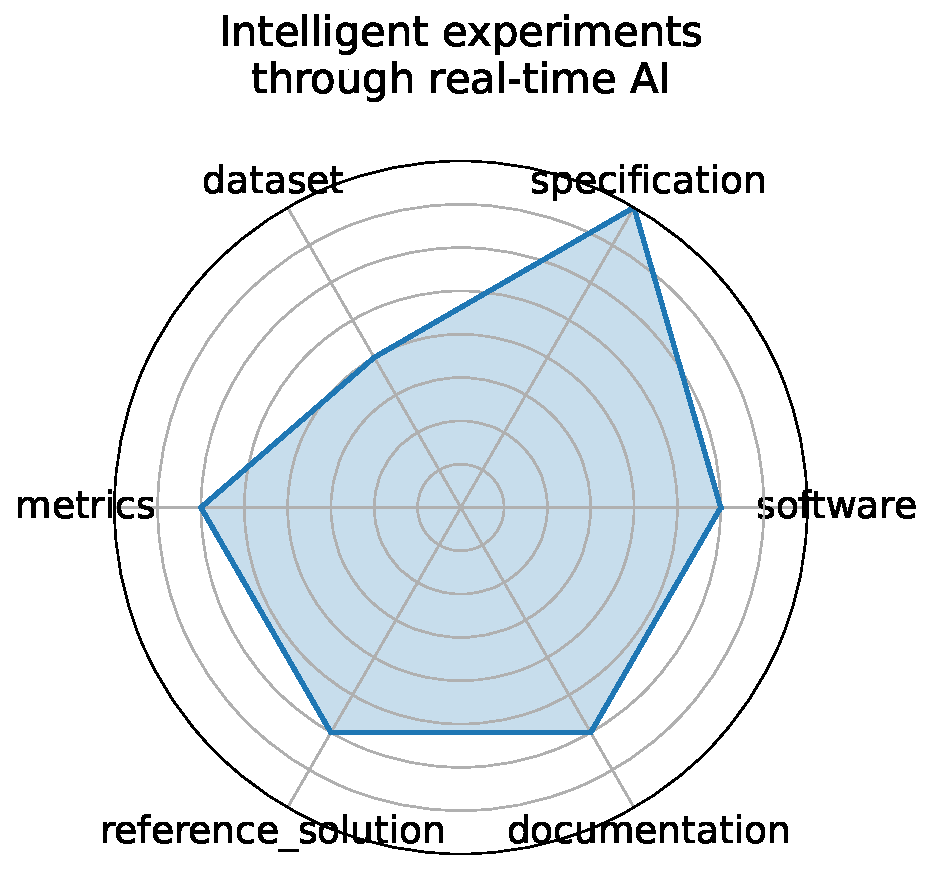
\includegraphics[width=0.15\textwidth]{intelligent_experiments_through_real-time_ai_radar.pdf} & Intelligent experiments through real-time AI & Instrumentation and Detectors; Nuclear Physics; Particle Physics & Real-time FPGA-based triggering and detector control for sPHENIX and future EIC & FPGA, Graph Neural Network, hls4ml, real-time inference, detector control & Trigger classification, Detector control, Real-time inference & Low-latency GNN inference on FPGA & Accuracy (charm and beauty detection), Latency (micros), Resource utilization (LUT/FF/BRAM/DSP) & Bipartite Graph Network with Set Transformers (BGN-ST), GarNet (edge-classifier) & \cite{kvapil2025intelligentexperimentsrealtimeai}\href{https://arxiv.org/pdf/2501.04845}{$\Rightarrow$} \\ \hline
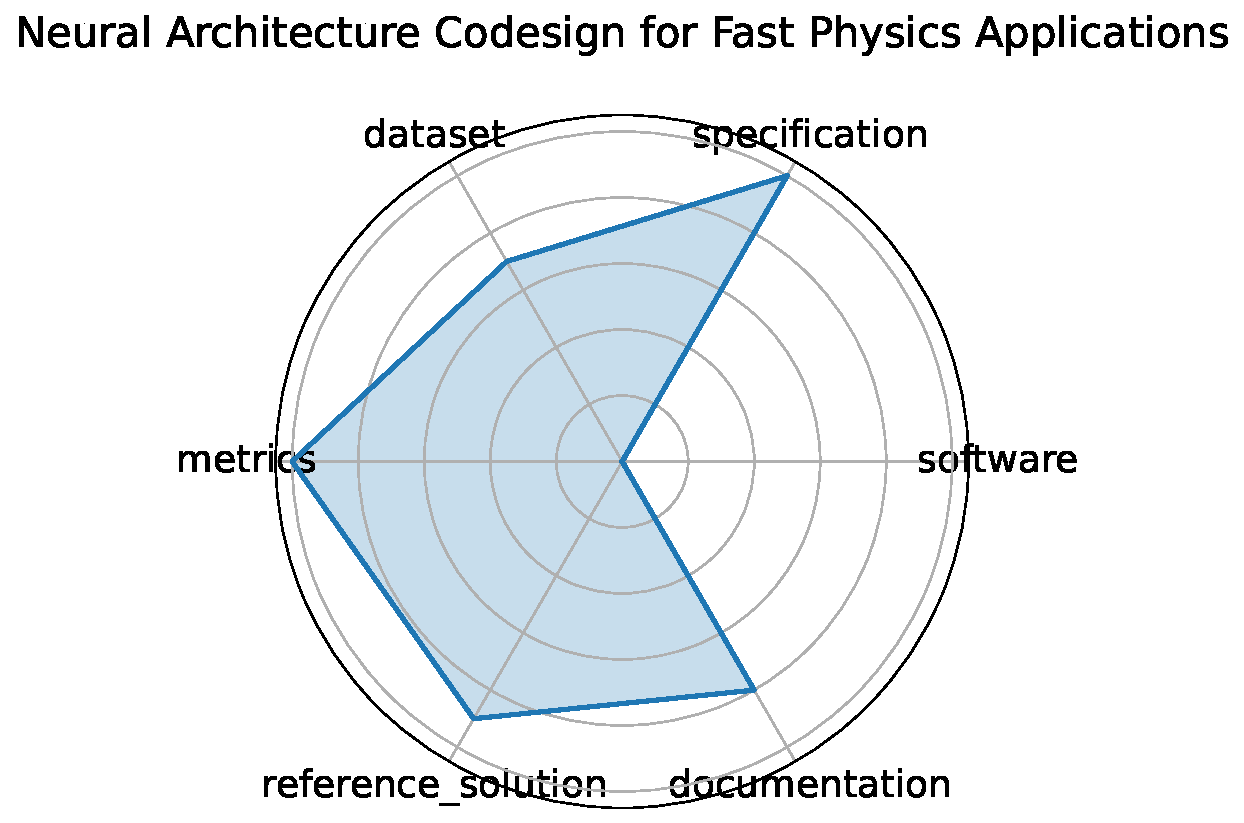
\includegraphics[width=0.15\textwidth]{neural_architecture_codesign_for_fast_physics_applications_radar.pdf} & Neural Architecture Codesign for Fast Physics Applications & Physics; Materials Science; Particle Physics & Automated neural architecture search and hardware-efficient model codesign for fast physics applications & neural architecture search, FPGA deployment, quantization, pruning, hls4ml & Classification, Peak finding & Hardware-aware model optimization; low-latency inference & Accuracy, Latency, Resource utilization & NAC-based BraggNN, NAC-optimized Deep Sets (jet) & \cite{weitz2025neuralarchitecturecodesignfast}\href{https://arxiv.org/abs/2501.05515}{$\Rightarrow$} \\ \hline
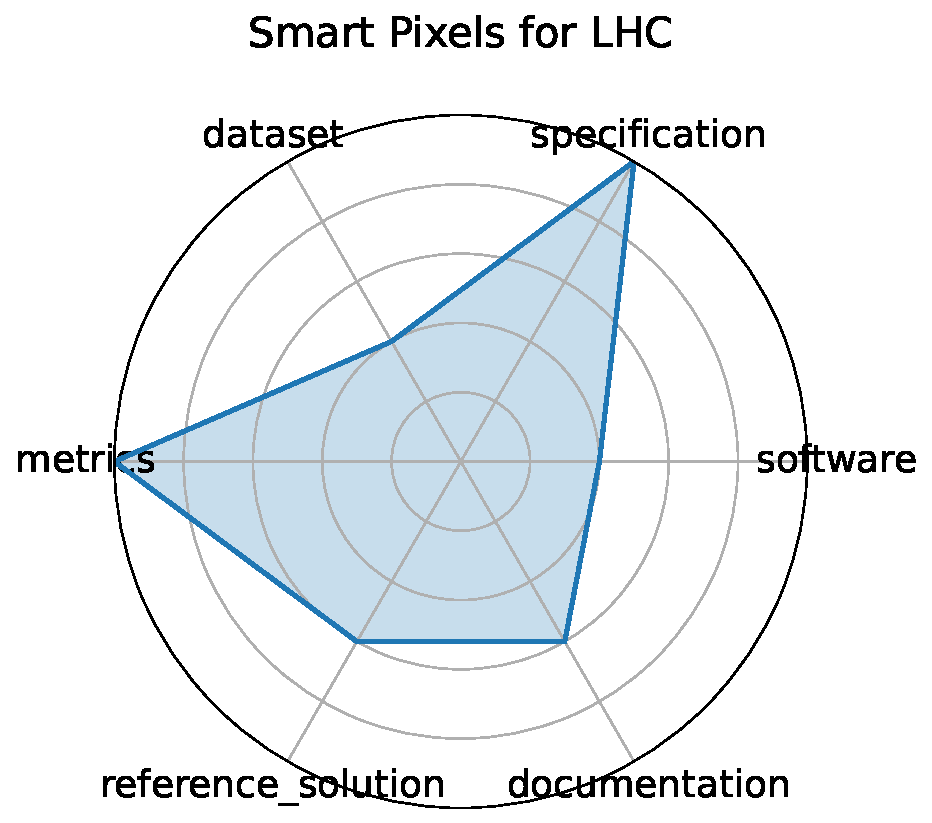
\includegraphics[width=0.15\textwidth]{smart_pixels_for_lhc_radar.pdf} & Smart Pixels for LHC & Particle Physics; Instrumentation and Detectors & On-sensor, in-pixel ML filtering for high-rate LHC pixel detectors & smart pixel, on-sensor inference, data reduction, trigger & Image Classification, Data filtering & On-chip, low-power inference; data reduction & Data rejection rate, Power per pixel & 2-layer pixel NN & \cite{parpillon2024smartpixelsinpixelai}\href{https://arxiv.org/abs/2406.14860}{$\Rightarrow$} \\ \hline
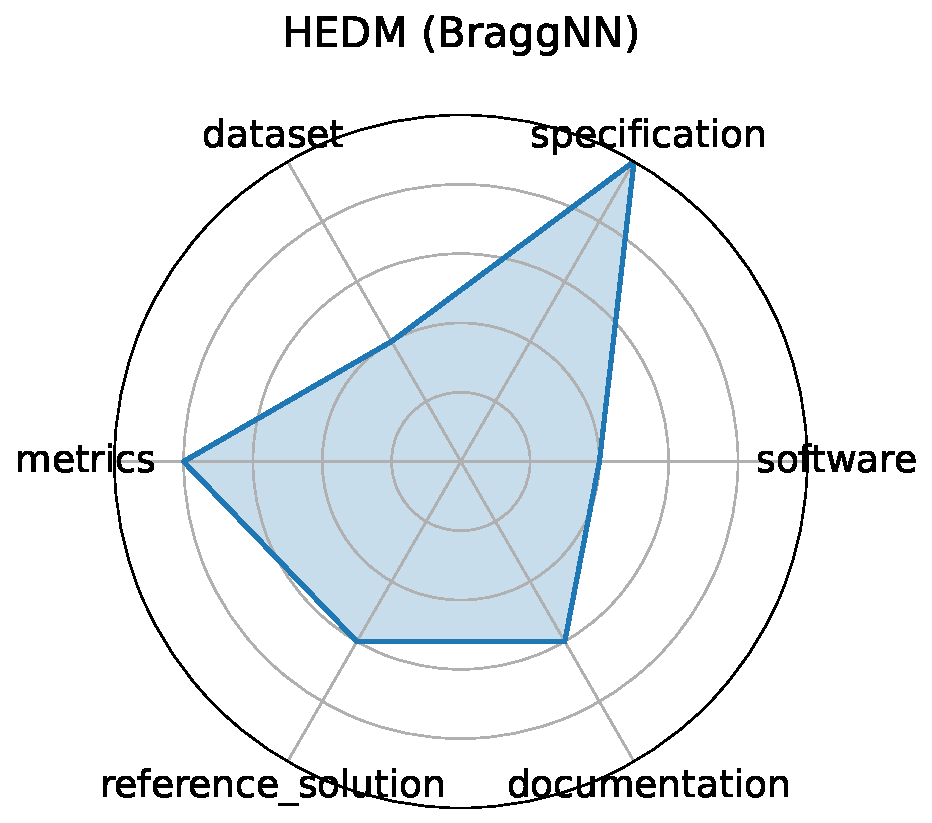
\includegraphics[width=0.15\textwidth]{hedm_braggnn_radar.pdf} & HEDM (BraggNN) & Material Science & Fast Bragg peak analysis using deep learning in diffraction microscopy & BraggNN, diffraction, peak finding, HEDM & Peak detection & High-throughput peak localization & Localization accuracy, Inference time & BraggNN & \cite{liu2021braggnnfastxraybragg}\href{https://arxiv.org/abs/2008.08198}{$\Rightarrow$} \\ \hline
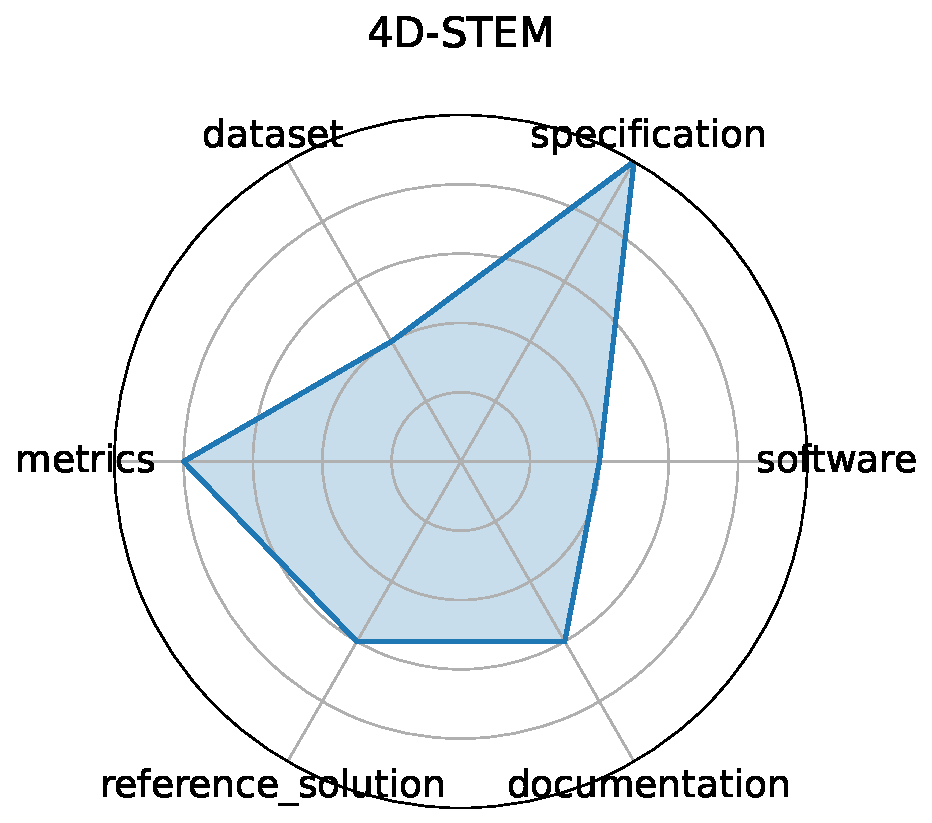
\includegraphics[width=0.15\textwidth]{d-stem_radar.pdf} & 4D-STEM & Material Science & Real-time ML for scanning transmission electron microscopy & 4D-STEM, electron microscopy, real-time, image processing & Image Classification, Streamed data inference & Real-time large-scale microscopy inference & Classification accuracy, Throughput & CNN models (prototype) & \cite{qin2023extremely}\href{https://openreview.net/pdf?id=7yt3N0o0W9}{$\Rightarrow$} \\ \hline
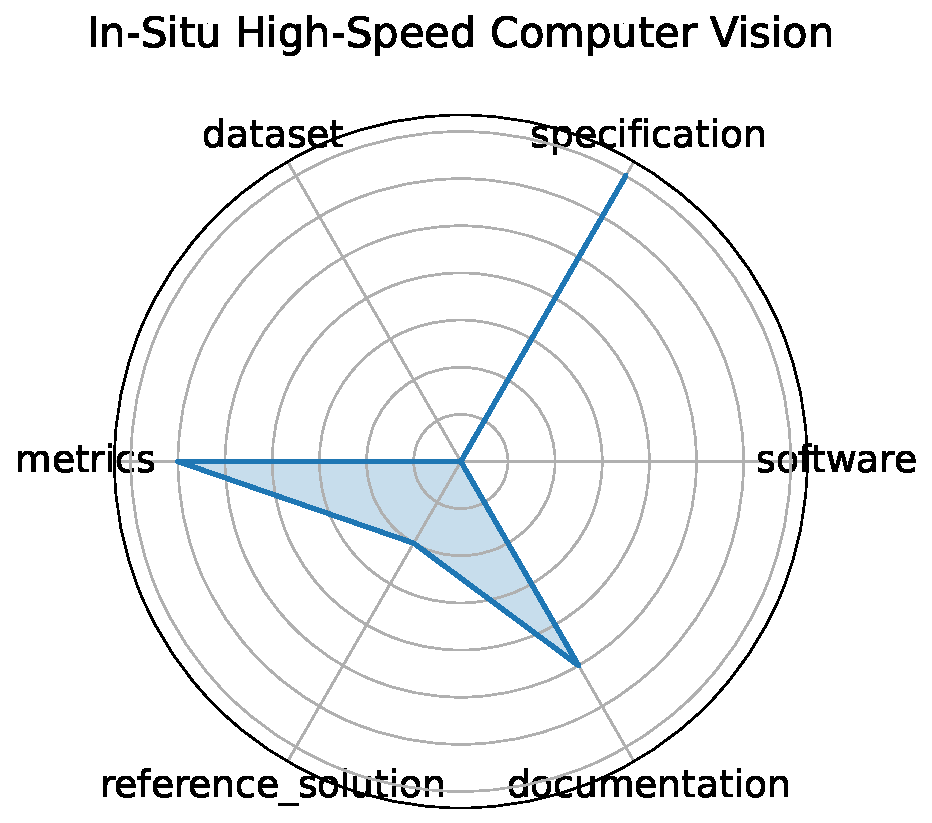
\includegraphics[width=0.15\textwidth]{in-situ_high-speed_computer_vision_radar.pdf} & In-Situ High-Speed Computer Vision & Fusion/Plasma & Real-time image classification for in-situ plasma diagnostics & plasma, in-situ vision, real-time ML & Image Classification & Real-time diagnostic inference & Accuracy, FPS & CNN & \cite{wei2024lowlatencyopticalbasedmode}\href{https://arxiv.org/abs/2312.00128}{$\Rightarrow$} \\ \hline
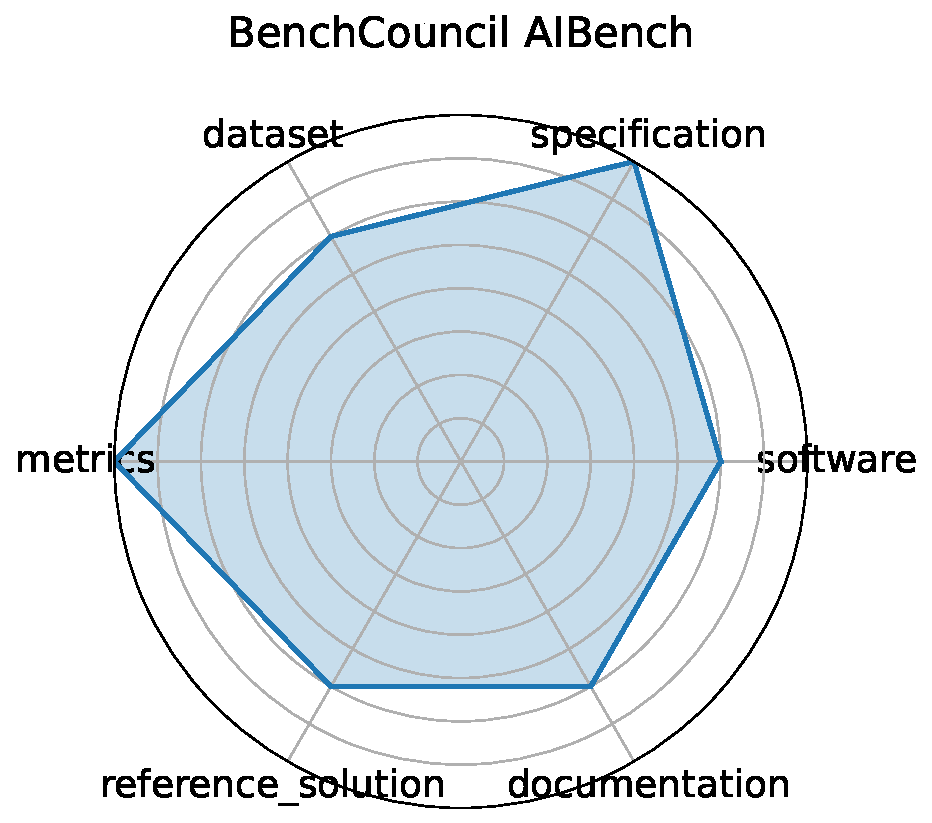
\includegraphics[width=0.15\textwidth]{benchcouncil_aibench_radar.pdf} & BenchCouncil AIBench & General & End-to-end AI benchmarking across micro, component, and application levels & benchmarking, AI systems, application-level evaluation & Training, Inference, End-to-end AI workloads & System-level AI workload performance & Throughput, Latency, Accuracy & ResNet, BERT, GANs, Recommendation systems & \cite{gao2019aibenchindustrystandardinternet}\href{https://www.benchcouncil.org/AIBench/}{$\Rightarrow$} \\ \hline
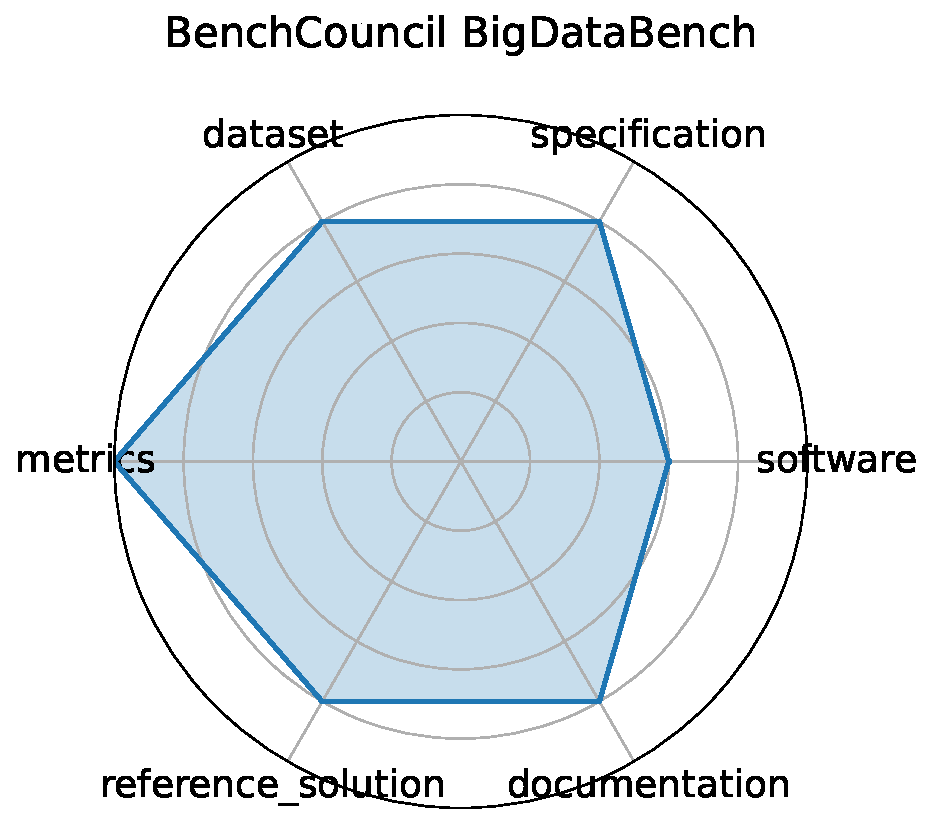
\includegraphics[width=0.15\textwidth]{benchcouncil_bigdatabench_radar.pdf} & BenchCouncil BigDataBench & General & Big data and AI benchmarking across structured, semi-structured, and unstructured data workloads & big data, AI benchmarking, data analytics & Data preprocessing, Inference, End-to-end data pipelines & Data processing and AI model inference performance at scale & Data throughput, Latency, Accuracy & CNN, LSTM, SVM, XGBoost & \cite{gao2018bigdatabenchscalableunifiedbig}\href{https://www.benchcouncil.org/BigDataBench/}{$\Rightarrow$} \\ \hline
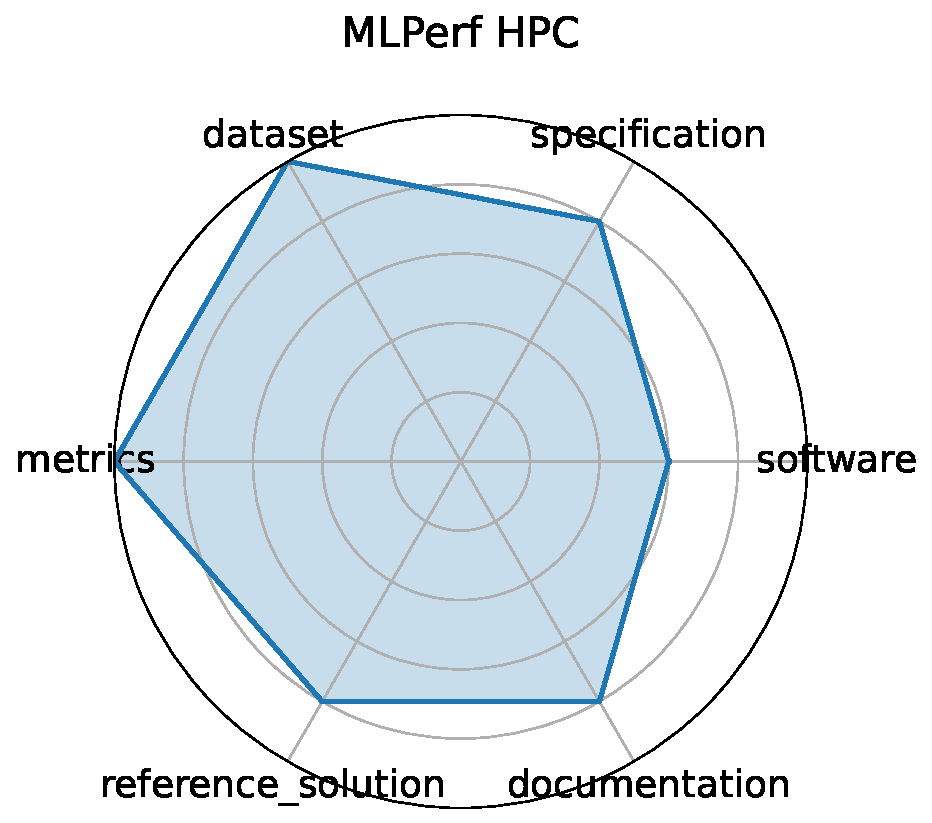
\includegraphics[width=0.15\textwidth]{mlperf_hpc_radar.pdf} & MLPerf HPC & Cosmology, Climate, Protein Structure, Catalysis & Scientific ML training and inference on HPC systems & HPC, training, inference, scientific ML & Training, Inference & Scaling efficiency, training time, model accuracy on HPC & Training time, Accuracy, GPU utilization & CosmoFlow, DeepCAM, OpenCatalyst & \cite{farrell2021mlperfhpcholisticbenchmark}\href{https://github.com/mlcommons/hpc}{$\Rightarrow$} \\ \hline
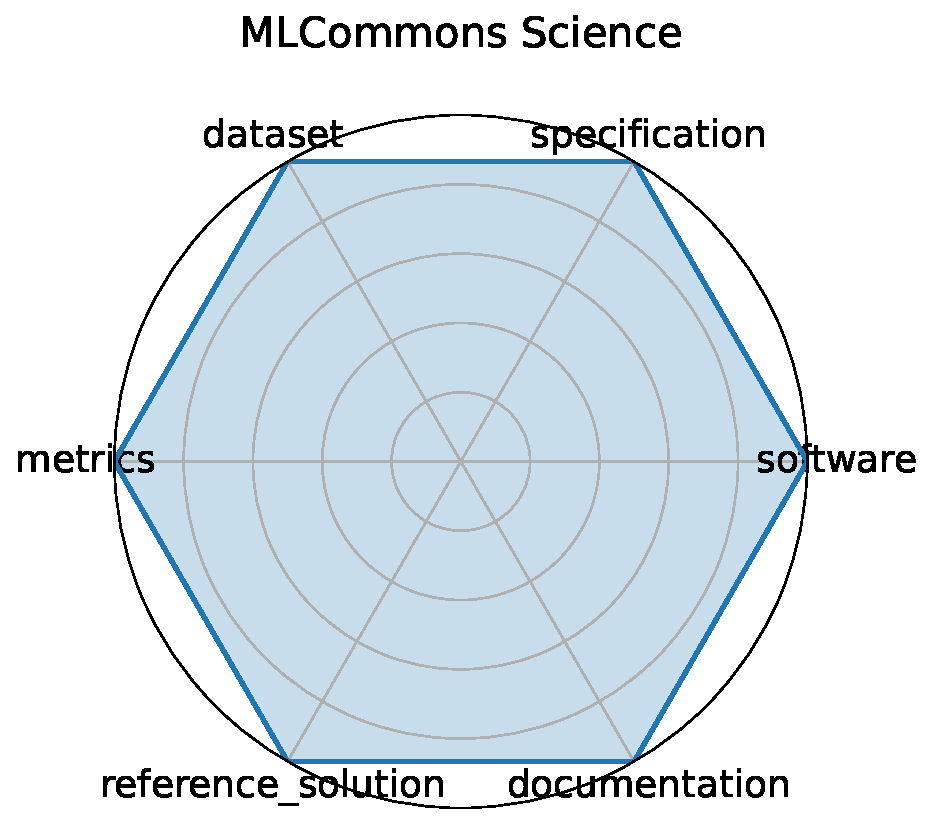
\includegraphics[width=0.15\textwidth]{mlcommons_science_radar.pdf} & MLCommons Science & Earthquake, Satellite Image, Drug Discovery, Electron Microscope, CFD & AI benchmarks for scientific applications including time-series, imaging, and simulation & science AI, benchmark, MLCommons, HPC & Time-series analysis, Image classification, Simulation surrogate modeling & Inference accuracy, simulation speed-up, generalization & MAE, Accuracy, Speedup vs simulation & CNN, GNN, Transformer & \cite{10.1007/978-3-031-23220-6_4}\href{https://github.com/mlcommons/science}{$\Rightarrow$} \\ \hline
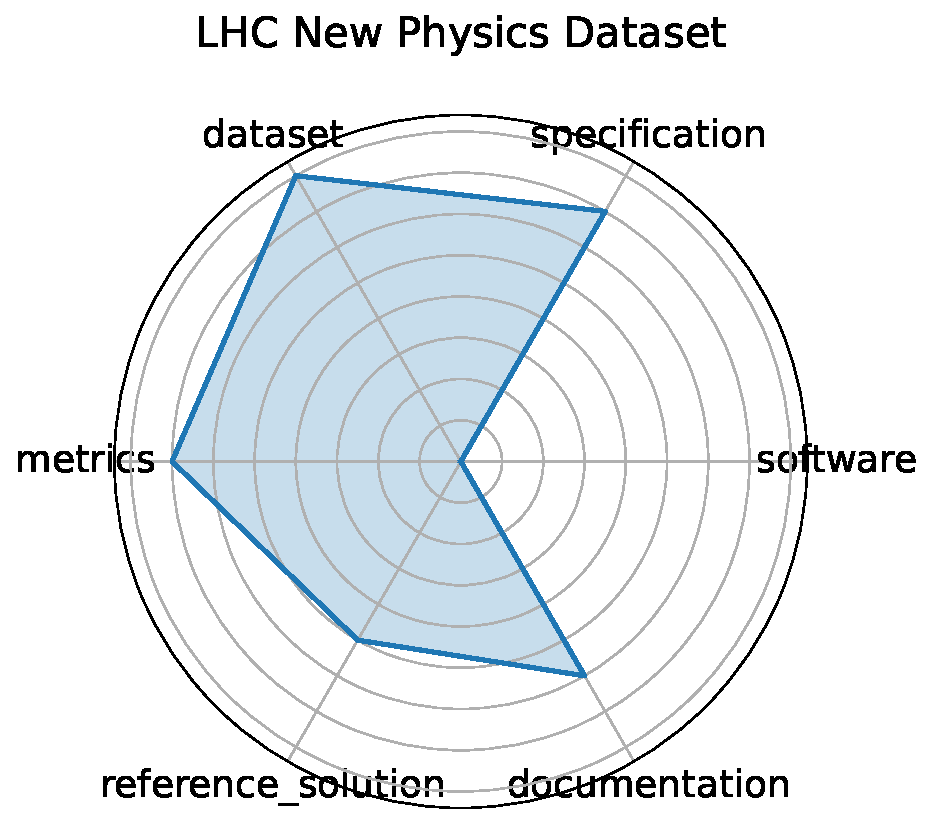
\includegraphics[width=0.15\textwidth]{lhc_new_physics_dataset_radar.pdf} & LHC New Physics Dataset & Particle Physics; Real-time Triggering & Real-time LHC event filtering for anomaly detection using proton collision data & anomaly detection, proton collision, real-time inference, event filtering, unsupervised ML & Anomaly detection, Event classification & Unsupervised signal detection under latency and bandwidth constraints & ROC-AUC, Detection efficiency & Autoencoder, Variational autoencoder, Isolation forest & \cite{https://doi.org/10.5281/zenodo.5046389}\href{https://arxiv.org/pdf/2107.02157}{$\Rightarrow$} \\ \hline
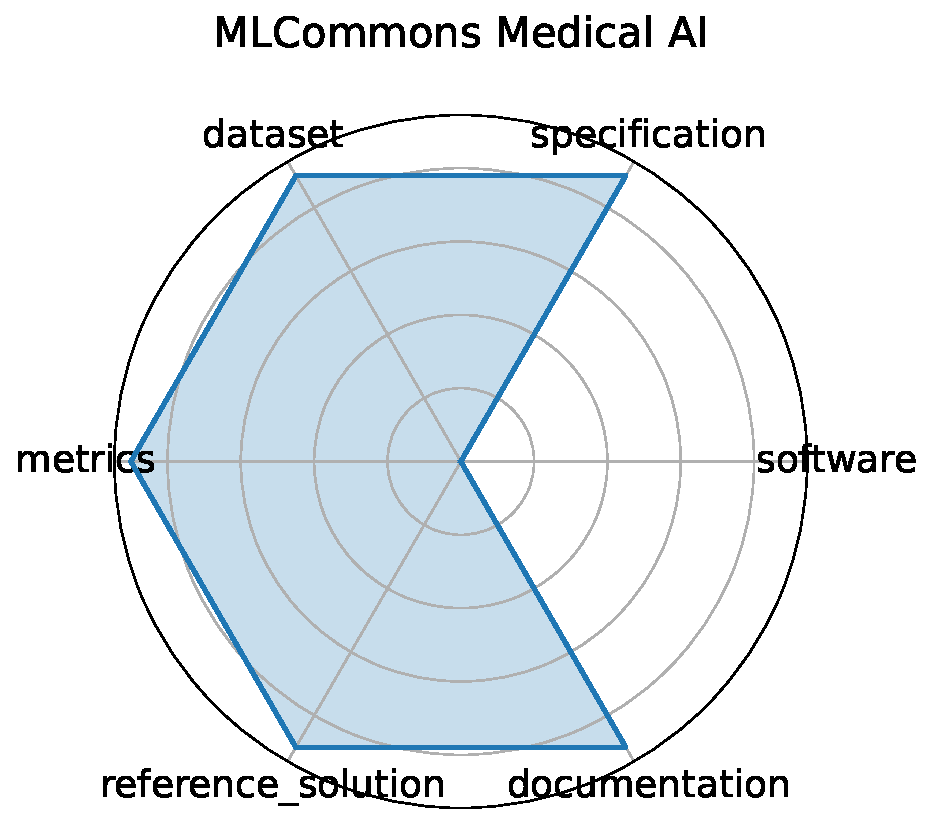
\includegraphics[width=0.15\textwidth]{mlcommons_medical_ai_radar.pdf} & MLCommons Medical AI & Healthcare; Medical AI & Federated benchmarking and evaluation of medical AI models across diverse real-world clinical data & medical AI, federated evaluation, privacy-preserving, fairness, healthcare benchmarks & Federated evaluation, Model validation & Clinical accuracy, fairness, generalizability, privacy compliance & ROC AUC, Accuracy, Fairness metrics & MedPerf-validated CNNs, GaNDLF workflows & \cite{karargyris2023federated}\href{https://github.com/mlcommons/medical}{$\Rightarrow$} \\ \hline
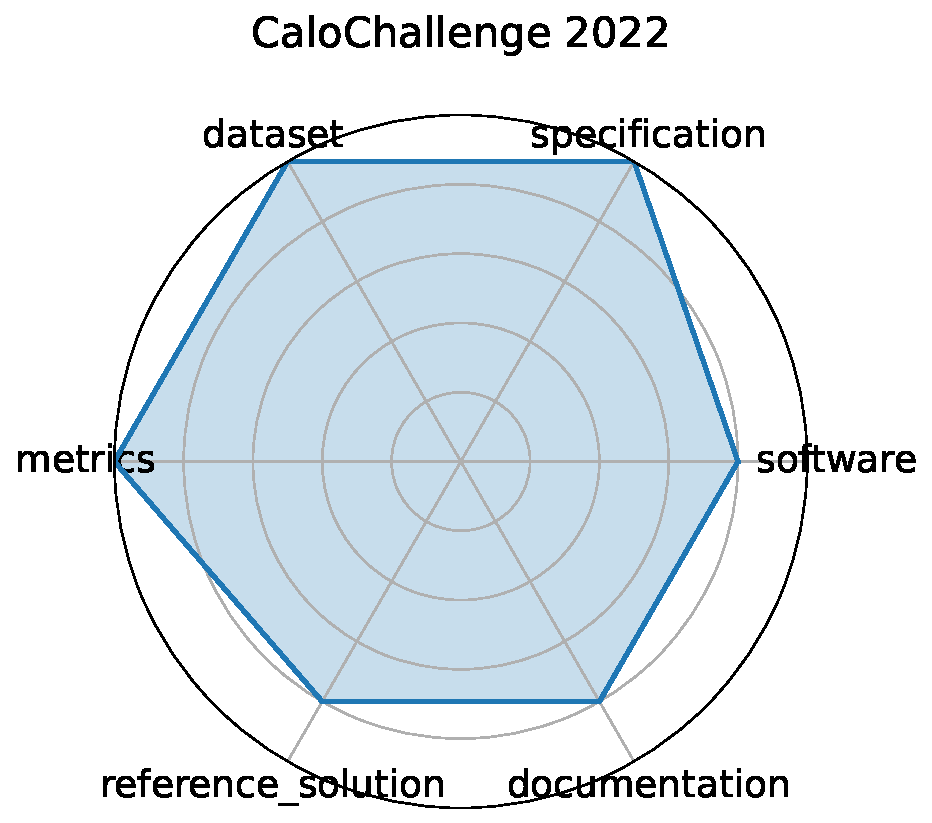
\includegraphics[width=0.15\textwidth]{calochallenge__radar.pdf} & CaloChallenge 2022 & LHC Calorimeter; Particle Physics & Fast generative-model-based calorimeter shower simulation evaluation & calorimeter simulation, generative models, surrogate modeling, LHC, fast simulation & Surrogate modeling & Simulation fidelity, speed, efficiency & Histogram similarity, Classifier AUC, Generation latency & VAE variants, GAN variants, Normalizing flows, Diffusion models & \cite{krause2024calochallenge2022communitychallenge}\href{http://arxiv.org/abs/2410.21611}{$\Rightarrow$} \\ \hline
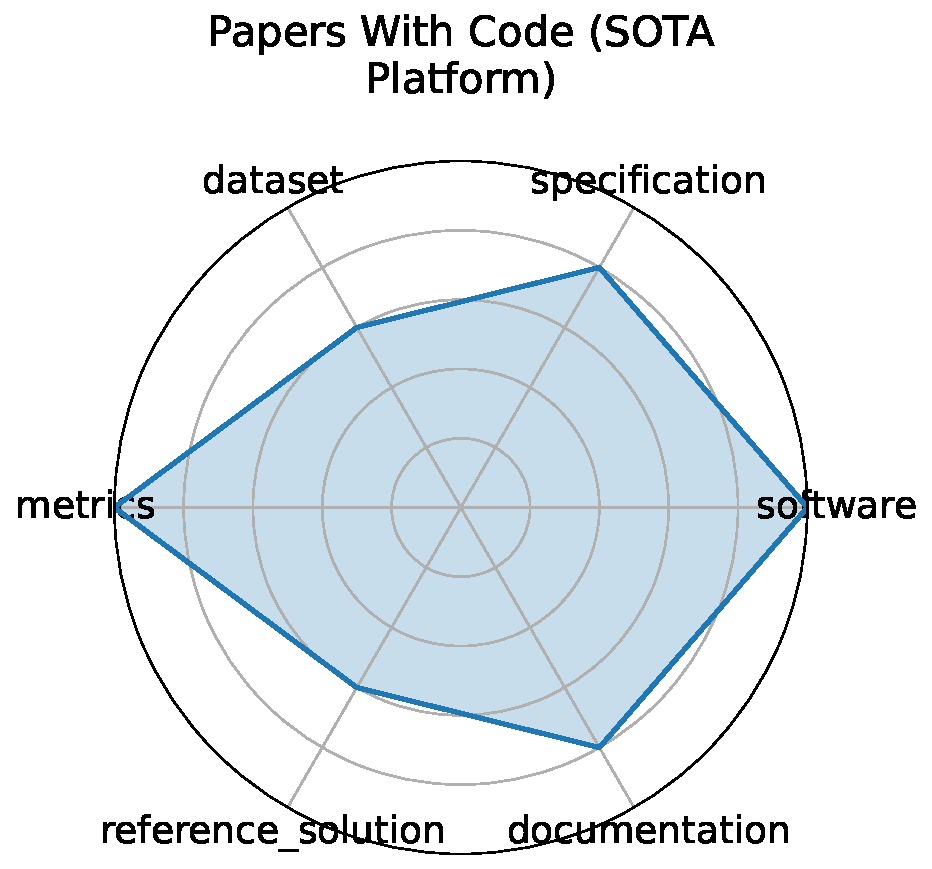
\includegraphics[width=0.15\textwidth]{papers_with_code_sota_platform_radar.pdf} & Papers With Code (SOTA Platform) & General ML; All domains & Open platform tracking state-of-the-art results, benchmarks, and implementations across ML tasks and papers & leaderboard, benchmarking, reproducibility, open-source & Multiple (Classification, Detection, NLP, etc.) & Model performance across tasks (accuracy, F1, BLEU, etc.) & Task-specific (Accuracy, F1, BLEU, etc.) & All published models with code & \cite{pmlr-v37-blum15}\href{https://paperswithcode.com/sota}{$\Rightarrow$} \\ \hline
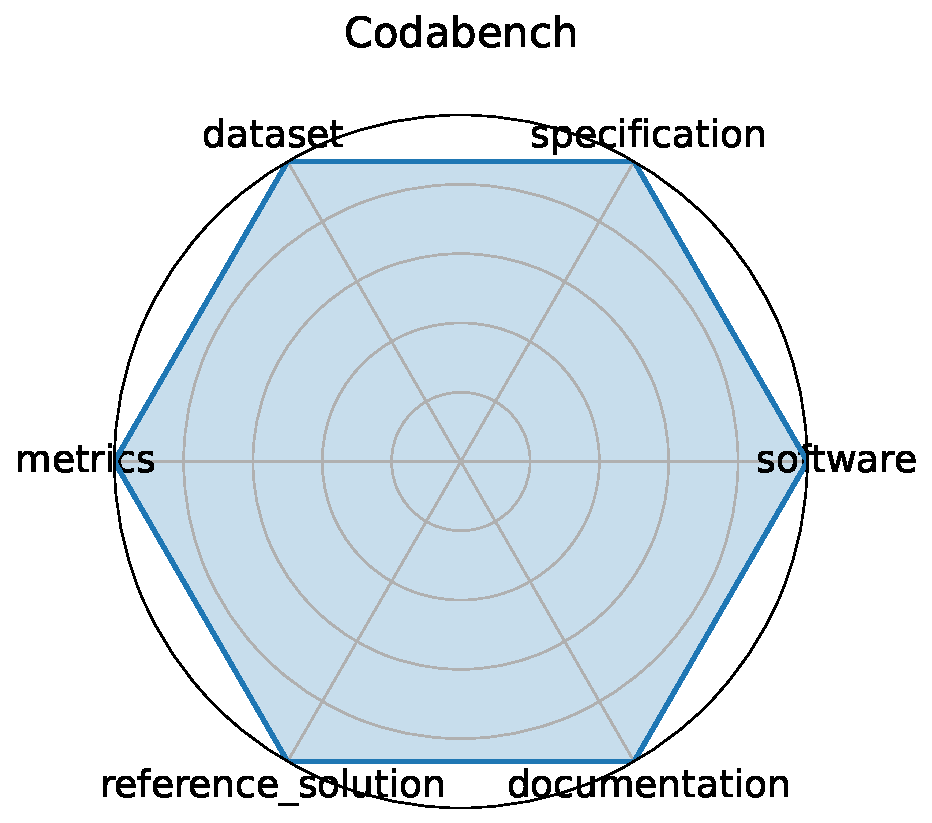
\includegraphics[width=0.15\textwidth]{codabench_radar.pdf} & Codabench & General ML; Multiple & Open-source platform for organizing reproducible AI benchmarks and competitions & benchmark platform, code submission, competitions, meta-benchmark & Multiple & Model reproducibility, performance across datasets & Submission count, Leaderboard ranking, Task-specific metrics & Arbitrary code submissions & \cite{xu-2022}\href{https://www.codabench.org/}{$\Rightarrow$} \\ \hline
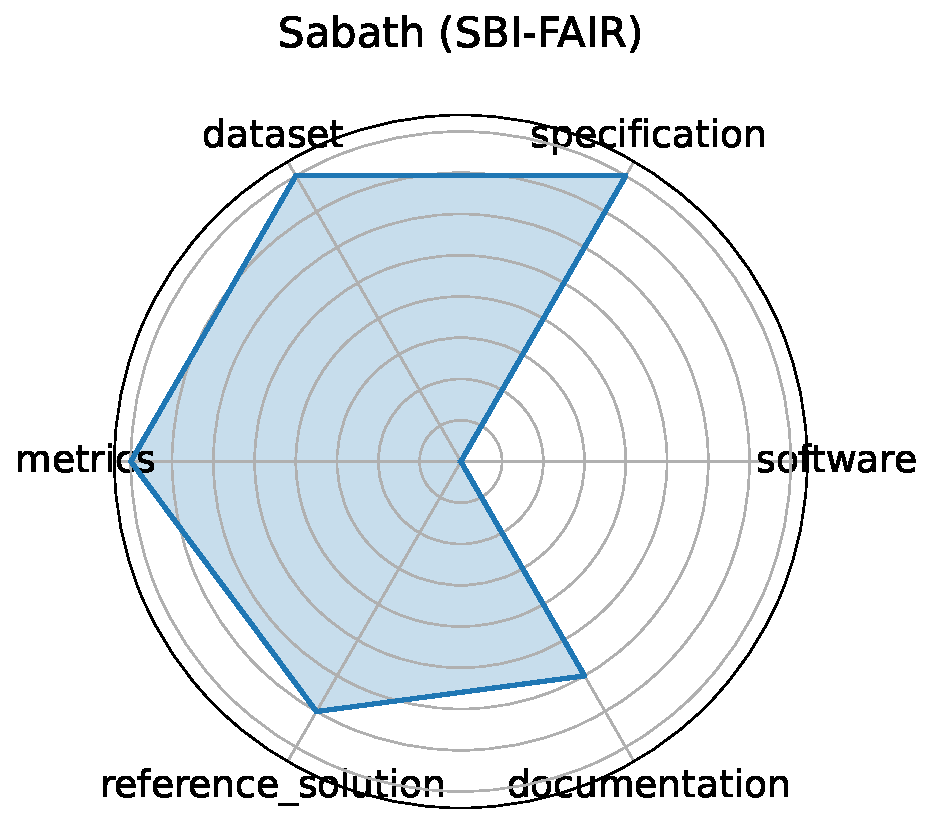
\includegraphics[width=0.15\textwidth]{sabath_sbi-fair_radar.pdf} & Sabath (SBI-FAIR) & Systems; Metadata & FAIR metadata framework for ML-driven surrogate workflows in HPC systems & meta-benchmark, metadata, HPC, surrogate modeling & Systems benchmarking & Metadata tracking, reproducible HPC workflows & Metadata completeness, FAIR compliance & NA & \cite{luszczek2021sabath}\href{https://sbi-fair.github.io/docs/software/sabath/}{$\Rightarrow$} \\ \hline
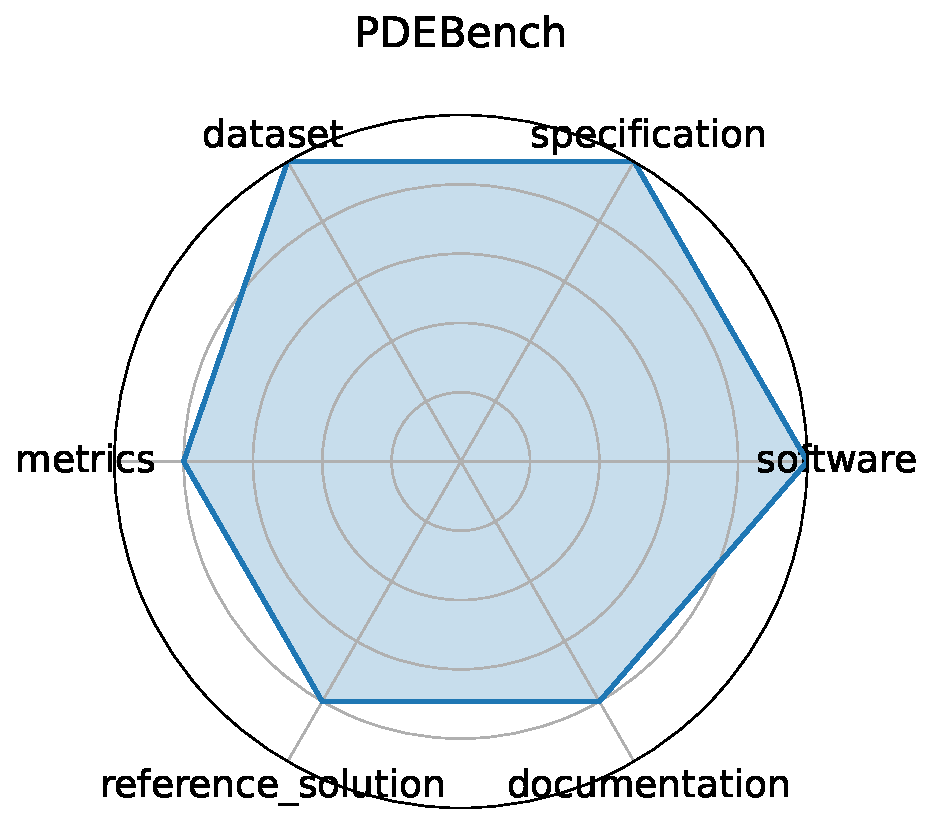
\includegraphics[width=0.15\textwidth]{pdebench_radar.pdf} & PDEBench & CFD; Weather Modeling & Benchmark suite for ML-based surrogates solving time-dependent PDEs & PDEs, CFD, scientific ML, surrogate modeling, NeurIPS & Supervised Learning & Time-dependent PDE modeling; physical accuracy & RMSE, boundary RMSE, Fourier RMSE & FNO, U-Net, PINN, Gradient-Based inverse methods & \cite{takamoto2024pdebenchextensivebenchmarkscientific}\href{https://github.com/pdebench/PDEBench}{$\Rightarrow$} \\ \hline
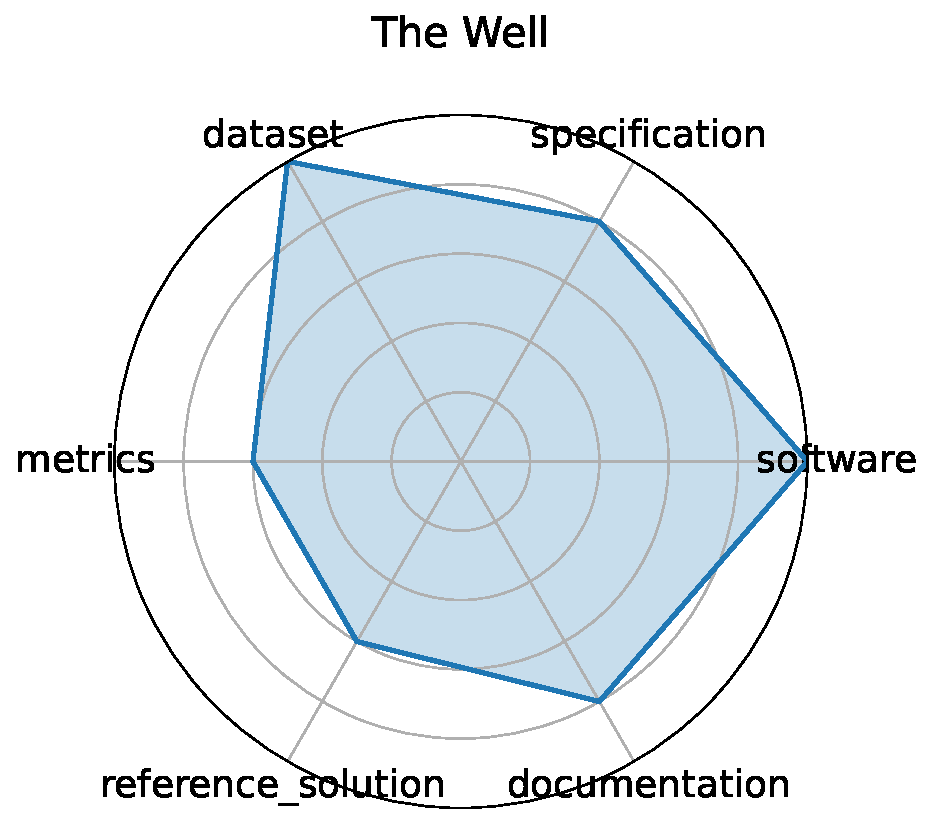
\includegraphics[width=0.15\textwidth]{the_well_radar.pdf} & The Well & biological systems, fluid dynamics, acoustic scattering, astrophysical MHD & Foundation model + surrogate dataset spanning 16 physical simulation domains & surrogate modeling, foundation model, physics simulations, spatiotemporal dynamics & Supervised Learning & Surrogate modeling, physics-based prediction & Dataset size, Domain breadth & FNO baselines, U-Net baselines & \cite{neurips2024_4f9a5acd}\href{https://polymathic-ai.org/the\_well/}{$\Rightarrow$} \\ \hline
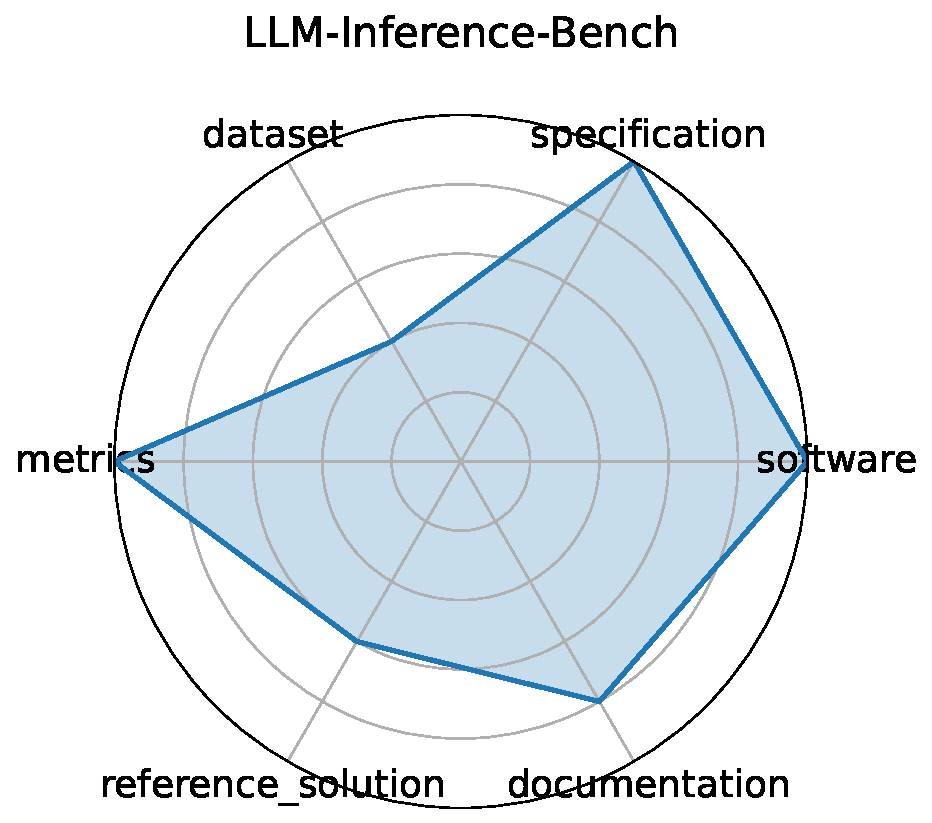
\includegraphics[width=0.15\textwidth]{llm-inference-bench_radar.pdf} & LLM-Inference-Bench & LLM; HPC/inference & Hardware performance benchmarking of LLMs on AI accelerators & LLM, inference benchmarking, GPU, accelerator, throughput & Inference Benchmarking & Inference throughput, latency, hardware utilization & Token throughput (tok/s), Latency, Framework-hardware mix performance & LLaMA-2-7B, LLaMA-2-70B, Mistral-7B, Qwen-7B & \cite{10820566}\href{https://github.com/argonne-lcf/LLM-Inference-Bench}{$\Rightarrow$} \\ \hline
\includegraphics[width=0.15\textwidth]{sglang_framework_radar.pdf} & SGLang Framework & LLM Vision & Fast serving framework for LLMs and vision-language models & LLM serving, vision-language, RadixAttention, performance, JSON decoding & Model serving framework & Serving throughput, JSON/task-specific latency & Tokens/sec, Time-to-first-token, Throughput gain vs baseline & LLaVA, DeepSeek, Llama & \cite{zheng2024sglangefficientexecutionstructured}\href{https://github.com/sgl-project/sglang/tree/main/benchmark}{$\Rightarrow$} \\ \hline
\includegraphics[width=0.15\textwidth]{vllm_inference_and_serving_engine_radar.pdf} & vLLM Inference and Serving Engine & LLM; HPC/inference & High-throughput, memory-efficient inference and serving engine for LLMs & LLM inference, PagedAttention, CUDA graph, streaming API, quantization & Inference Benchmarking & Throughput, latency, memory efficiency & Tokens/sec, Time to First Token (TTFT), Memory footprint & LLaMA, Mixtral, FlashAttention-based models & \cite{10.1145/3600006.3613165}\href{https://github.com/vllm-project/vllm/tree/main/benchmarks}{$\Rightarrow$} \\ \hline
\includegraphics[width=0.15\textwidth]{vllm_performance_dashboard_radar.pdf} & vLLM Performance Dashboard & LLM; HPC/inference & Interactive dashboard showing inference performance of vLLM & Dashboard, Throughput visualization, Latency analysis, Metric tracking & Performance visualization & Throughput, latency, hardware utilization & Tokens/sec, TTFT, Memory usage & LLaMA-2, Mistral, Qwen & \cite{mo2024vllm_dashboard}\href{https://simon-mo-workspace.observablehq.cloud/vllm-dashboard-v0/}{$\Rightarrow$} \\ \hline
\includegraphics[width=0.15\textwidth]{nixtla_neuralforecast_radar.pdf} & Nixtla NeuralForecast & Time-series forecasting; General ML & High-performance neural forecasting library with \ensuremath{>}30 models & time-series, neural forecasting, NBEATS, NHITS, TFT, probabilistic forecasting, usability & Time-series forecasting & Forecast accuracy, interpretability, speed & RMSE, MAPE, CRPS & NBEATS, NHITS, TFT, DeepAR & \cite{olivares2022library_neuralforecast}\href{https://github.com/Nixtla/neuralforecast}{$\Rightarrow$} \\ \hline
\includegraphics[width=0.15\textwidth]{nixtla_neural_forecast_nhits_radar.pdf} & Nixtla Neural Forecast NHITS & Time-series; General ML & Official NHITS implementation for long-horizon time series forecasting & NHITS, long-horizon forecasting, neural interpolation, time-series & Time-series forecasting & Accuracy, compute efficiency for long series & RMSE, MAPE & NHITS & \cite{challu2023nhits}\href{https://github.com/Nixtla/neuralforecast}{$\Rightarrow$} \\ \hline
\includegraphics[width=0.15\textwidth]{nixtla_neural_forecast_timellm_radar.pdf} & Nixtla Neural Forecast TimeLLM & Time-series; General ML & Reprogramming LLMs for time series forecasting & Time-LLM, language model, time-series, reprogramming & Time-series forecasting & Model reuse via LLM, few-shot forecasting & RMSE, MAPE & Time-LLM & \cite{jin2024timellmtimeseriesforecasting}\href{https://github.com/Nixtla/neuralforecast}{$\Rightarrow$} \\ \hline
\includegraphics[width=0.15\textwidth]{nixtla_neural_forecast_timegpt_radar.pdf} & Nixtla Neural Forecast TimeGPT & Time-series; General ML & Time-series foundation model ''TimeGPT'' for forecasting and anomaly detection & TimeGPT, foundation model, time-series, generative model & Time-series forecasting, Anomaly detection & Zero-shot forecasting, anomaly detection & RMSE, Anomaly detection metrics & TimeGPT & \cite{garza2024timegpt1}\href{https://github.com/Nixtla/neuralforecast}{$\Rightarrow$} \\ \hline
\includegraphics[width=0.15\textwidth]{hdr_ml_anomaly_challenge_gravitational_waves_radar.pdf} & HDR ML Anomaly Challenge (Gravitational Waves) & Astrophysics; Time-series & Detecting anomalous gravitational-wave signals from LIGO/Virgo datasets & anomaly detection, gravitational waves, astrophysics, time-series & Anomaly detection & Novel event detection in physical signals & ROC-AUC, Precision/Recall & Deep latent CNNs, Autoencoders & \cite{campolongo2025buildingmachinelearningchallenges}\href{https://www.codabench.org/competitions/2626/}{$\Rightarrow$} \\ \hline
\includegraphics[width=0.15\textwidth]{hdr_ml_anomaly_challenge_butterfly_radar.pdf} & HDR ML Anomaly Challenge (Butterfly) & Genomics; Image/CV & Detecting hybrid butterflies via image anomaly detection in genomic-informed dataset & anomaly detection, computer vision, genomics, butterfly hybrids & Anomaly detection & Hybrid detection in biological systems & Classification accuracy, F1 score & CNN-based detectors & \cite{campolongo2025buildingmachinelearningchallenges2}\href{https://www.codabench.org/competitions/3764/}{$\Rightarrow$} \\ \hline
\includegraphics[width=0.15\textwidth]{hdr_ml_anomaly_challenge_sea_level_rise_radar.pdf} & HDR ML Anomaly Challenge (Sea Level Rise) & Climate Science; Time-series, Image/CV & Detecting anomalous sea-level rise and flooding events via time-series and satellite imagery & anomaly detection, climate science, sea-level rise, time-series, remote sensing & Anomaly detection & Detection of environmental anomalies & ROC-AUC, Precision/Recall & CNNs, RNNs, Transformers & \cite{campolongo2025buildingmachinelearningchallenges3}\href{https://www.codabench.org/competitions/3223/}{$\Rightarrow$} \\ \hline
\includegraphics[width=0.15\textwidth]{single_qubit_readout_on_qick_system_radar.pdf} & Single Qubit Readout on QICK System & Quantum Computing & Real-time single-qubit state classification using FPGA firmware & qubit readout, hls4ml, FPGA, QICK & Classification & Single-shot fidelity, inference latency & Accuracy, Latency & hls4ml quantized NN & \cite{diguglielmo2025endtoendworkflowmachinelearningbased}\href{https://github.com/fastmachinelearning/ml-quantum-readout}{$\Rightarrow$} \\ \hline
\includegraphics[width=0.15\textwidth]{gpqa_a_graduate-level_google-proof_question_and_answer_benchmark_radar.pdf} & GPQA: A Graduate-Level Google-Proof Question and Answer Benchmark & Science (Biology, Physics, Chemistry) & Graduate-level, expert-validated multiple-choice questions hard even with web access & Google-proof, multiple-choice, expert reasoning, science QA & Multiple choice & Scientific reasoning, knowledge probing & Accuracy & GPT-4 baseline & \cite{rein2023gpqagraduatelevelgoogleproofqa2}\href{https://arxiv.org/abs/2311.12022}{$\Rightarrow$} \\ \hline
\includegraphics[width=0.15\textwidth]{seafloorai_radar.pdf} & SeafloorAI & Marine Science; Vision-Language & Large-scale vision-language dataset for seafloor mapping and geological classification & sonar imagery, vision-language, seafloor mapping, segmentation, QA & Image segmentation, Vision-language QA & Geospatial understanding, multimodal reasoning & Segmentation pixel accuracy, QA accuracy & SegFormer, ViLT-style multimodal models & \cite{nguyen2024seafloor}\href{https://neurips.cc/virtual/2024/poster/97432}{$\Rightarrow$} \\ \hline
\includegraphics[width=0.15\textwidth]{supercond_radar.pdf} & SuperCon3D & Materials Science; Superconductivity & Dataset and models for predicting and generating high-Tc superconductors using 3D crystal structures & superconductivity, crystal structures, equivariant GNN, generative models & Regression (Tc prediction), Generative modeling & Structure-to-property prediction, structure generation & MAE (Tc), Validity of generated structures & SODNet, DiffCSP-SC & \cite{neurips2024_c4e3b55e}\href{https://neurips.cc/virtual/2024/poster/97553}{$\Rightarrow$} \\ \hline
\includegraphics[width=0.15\textwidth]{gess_radar.pdf} & GeSS & Scientific ML; Geometric Deep Learning & Benchmark suite evaluating geometric deep learning models under real-world distribution shifts & geometric deep learning, distribution shift, OOD robustness, scientific applications & Classification, Regression & OOD performance in scientific settings & Accuracy, RMSE, OOD robustness delta & GCN, EGNN, DimeNet++ & \cite{neurips2024_a8063075}\href{https://neurips.cc/virtual/2024/poster/97816}{$\Rightarrow$} \\ \hline
\includegraphics[width=0.15\textwidth]{vocal_call_locator_vcl_radar.pdf} & Vocal Call Locator (VCL) & Neuroscience; Bioacoustics & Benchmarking sound-source localization of rodent vocalizations from multi-channel audio & source localization, bioacoustics, time-series, SSL & Sound source localization & Source localization accuracy in bioacoustic settings & Localization error (cm), Recall/Precision & CNN-based SSL models & \cite{neurips2024_c00d37d6}\href{https://neurips.cc/virtual/2024/poster/97470}{$\Rightarrow$} \\ \hline
\includegraphics[width=0.15\textwidth]{massspecgym_radar.pdf} & MassSpecGym & Cheminformatics; Molecular Discovery & Benchmark suite for discovery and identification of molecules via MS/MS & mass spectrometry, molecular structure, de novo generation, retrieval, dataset & De novo generation, Retrieval, Simulation & Molecular identification and generation from spectral data & Structure accuracy, Retrieval precision, Simulation MSE & Graph-based generative models, Retrieval baselines & \cite{neurips2024_c6c31413}\href{https://neurips.cc/virtual/2024/poster/97823}{$\Rightarrow$} \\ \hline
\includegraphics[width=0.15\textwidth]{urban_data_layer_udl_radar.pdf} & Urban Data Layer (UDL) & Urban Computing; Data Engineering & Unified data pipeline for multi-modal urban science research & data pipeline, urban science, multi-modal, benchmark & Prediction, Classification & Multi-modal urban inference, standardization & Task-specific accuracy or RMSE & Baseline regression/classification pipelines & \cite{neurips2024_0db7f135}\href{https://neurips.cc/virtual/2024/poster/97837}{$\Rightarrow$} \\ \hline
\includegraphics[width=0.15\textwidth]{delta_squared-dft_radar.pdf} & Delta Squared-DFT & Computational Chemistry; Materials Science & Benchmarking machine-learning corrections to DFT using Delta Squared-trained models for reaction energies & density functional theory, Delta Squared-ML correction, reaction energetics, quantum chemistry & Regression & High-accuracy energy prediction, DFT correction & Mean Absolute Error (eV), Energy ranking accuracy & Delta Squared-ML correction networks, Kernel ridge regression & \cite{khrabrov2024nabla2dftuniversalquantumchemistry}\href{https://neurips.cc/virtual/2024/poster/97788}{$\Rightarrow$} \\ \hline
\includegraphics[width=0.15\textwidth]{llms_for_crop_science_radar.pdf} & LLMs for Crop Science & Agricultural Science; NLP & Evaluating LLMs on crop trait QA and textual inference tasks with domain-specific prompts & crop science, prompt engineering, domain adaptation, question answering & Question Answering, Inference & Scientific knowledge, crop reasoning & Accuracy, F1 score & GPT-4, LLaMA-2-13B, T5-XXL & \cite{shen2024exploringuserretrievalintegration}\href{https://neurips.cc/virtual/2024/poster/97570}{$\Rightarrow$} \\ \hline
\includegraphics[width=0.15\textwidth]{spiqa_llm_radar.pdf} & SPIQA (LLM) & Multimodal Scientific QA; Computer Vision & Evaluating LLMs on image-based scientific paper figure QA tasks (LLM Adapter performance) & multimodal QA, scientific figures, image+text, chain-of-thought prompting & Multimodal QA & Visual reasoning, scientific figure understanding & Accuracy, F1 score & LLaVA, MiniGPT-4, Owl-LLM adapter variants & \cite{pramanick2025spiqadatasetmultimodalquestion}\href{https://neurips.cc/virtual/2024/poster/97575}{$\Rightarrow$} \\ \hline
\end{longtable}
}

\end{landscape}
